\cleartooddpage[\thispagestyle{empty}]
\chapter{Gamma Ray Reconstruction}\label{ch:grrecon}

In chapter \ref{chapter:veritas}, it was explained how the trigger system preserves PMT voltage traces of potential events.
To reconstruct gamma rays, the voltage traces caused by cherenkov photons must be identified and combined to form an image of the original cherenkov shower.
Then the shower images from multiple telescopes can be used to reconstruct the original gamma ray's energy and direction.

\section{Pedestal Variation}
  Before reconstructing any events, the pedestal and pedestal variations (pedvars) must be calculated.
  These are done by artificially triggering all pixels once per second during observations, in order to record events that contain only noise.
  The average of the digital counts (dc) of all noise-events for each pixel is then the pedestal.
  From this pedestal, the pedvars are then calculated as the rms of the all the dc counts in all noise-events, which can be visualized as the distribution of dc around the mean dc.

\section{Pixel Identification}
  The first step is to determine which pixels are part of a shower image.
  This is done by subtracting the digital counts pedestal from the entire trace, and then integrating the total dc in each voltage trace.

  The start of a potential voltage pulse is the time when the voltage trace is at half of its maximum value, called $T_{0}$.
  Around time $T_{0}$, the trace is integrated a second time with a smaller time window (usually either 14 or 24 ns wide, at $T_0$ - 30\% of the window size), to reduce the inclusion of dc from sources of noise (NSB and electronics).
  This two-pass algorithm is usually referred to as the double-pass method\cite{doublepass}.
  If a pixel's second-pass total dc is higher than 5 times the pedvar, then it is considered an image pixel.
  If it is between 2.5 and 5 times the pedvar, it is considered a border pixel.

  Once all pixels have been classified, isolated border pixels that have no neighboring image pixel are removed from the image, as they are more likely to be due to noise than cherenkov photons.
  Then, the time gradient from the image and border pixels can be found by performing a linear fit of the $T_{0}$ times.
  This time gradient can then be used to place a (more accurate) third integration window with 30\% of the window before each pixel's $T_{0}$, to more accurately measure the charge due to cherenkov photons in the pixel.

  From the image pixels, border pixels, and time gradient, the shower's Hillas parameters \cite{hillas_params} can be calculated.
  These include the size of the shower in photoelectrons (or equivalent units), the shower center of charge, angle, length and width.
  The center of charge is the charge-weighted average of all image and border pixel positions.
  The angle of the shower determines how the image's major axis is oriented in the camera.
  The shower length and width are determined by the rms of the shower image along its major and minor axes, respectively.

\section{Position Reconstruction}\label{subsec:posrecon}
  By examining the images from multiple telescopes, the initial position of the event can be determined.
  This is done by overlapping all telescope images in a single camera coordinate system, and projecting each image's major axis backwards in time.
  These drawn lines should intersect very close together, and the average of the intersection points determines the event's initial direction.

  In averaging the intersection points, weighting for each intersection can be applied based on the angle between the two lines.
  This improves the reconstruction, because the intersection point from two images at \SI{90}{\degree} angles will be less sensitive to image fluctuations than two images at 160\degree, as shown in Figure \ref{fig:largeintersectangle}.
  Additionally, the disp method described in section \ref{subsec:disp} can be utilized to offer improvements at lower telescope elevations.

  \begin{figure}[ht]
    \begin{center}
      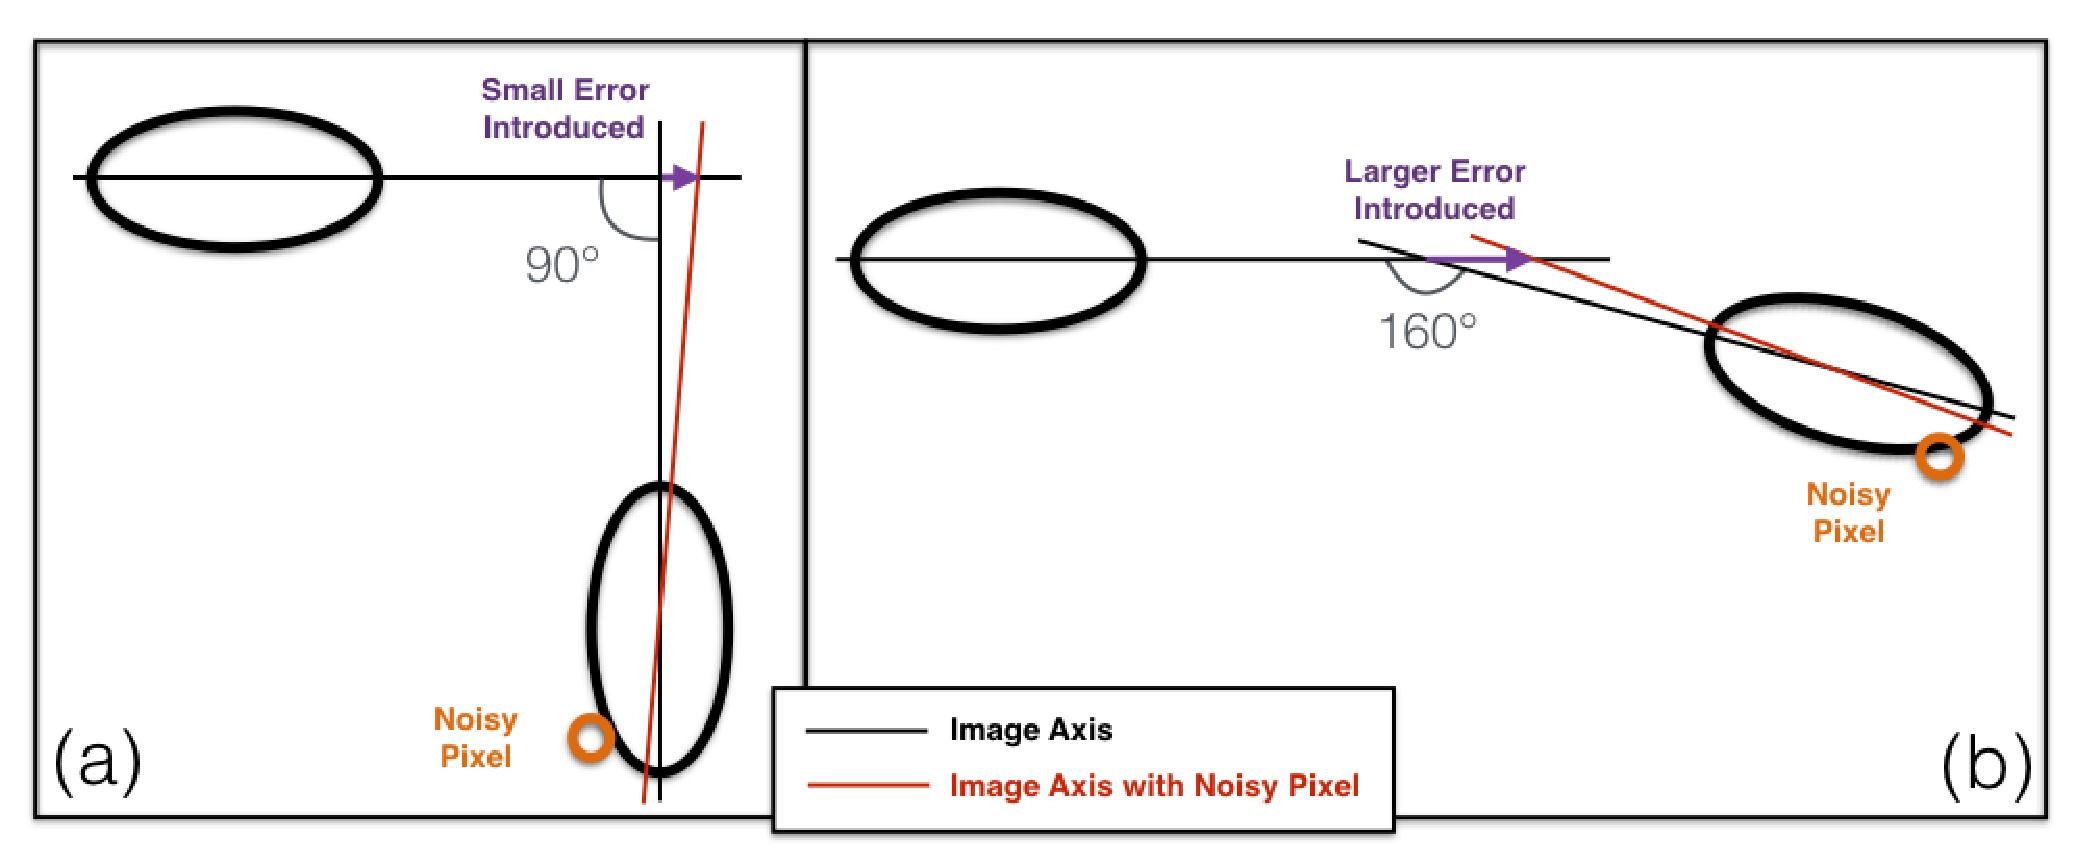
\includegraphics[width=0.95\textwidth]{images/large_angle_image_intersection_error_cropped.eps}
      \caption[Large Image Intersection Angles]{In diagram (a), when a noisy pixel is added to an image, the reconstructed position is only moved a small distance (the purple arrow).  In diagram (b), due to the large angle between images, the error in the reconstructed position is much larger.}\label{fig:largeintersectangle}
    \end{center}
  \end{figure}

  \subsection{Angular Reconstruction Neural Network}\label{subsec:disp}
    At high elevations, shower images often form small intesection angles, because the telescopes are spread out in two dimensions, relative to the shower in the atmosphere.
    At low elevations near the galactic center, however, the telescope array flattens into one dimension, which makes the shower's impact parameter (the shortest distance between the telescope and the shower core axis) smaller for two of the telescopes.
    These two closer telescopes then have very short, almost circular images, which increases the sensitivity of those two image axes to noisy pixels or shower fluctuations, as shown in Figure \ref{fig:showerhighlowelev}.
    This also causes the remaining telescope images to have large intersection angles, which also reduces the accuracy of the position reconstruction.

    \begin{figure}[ht]
      \begin{center}
        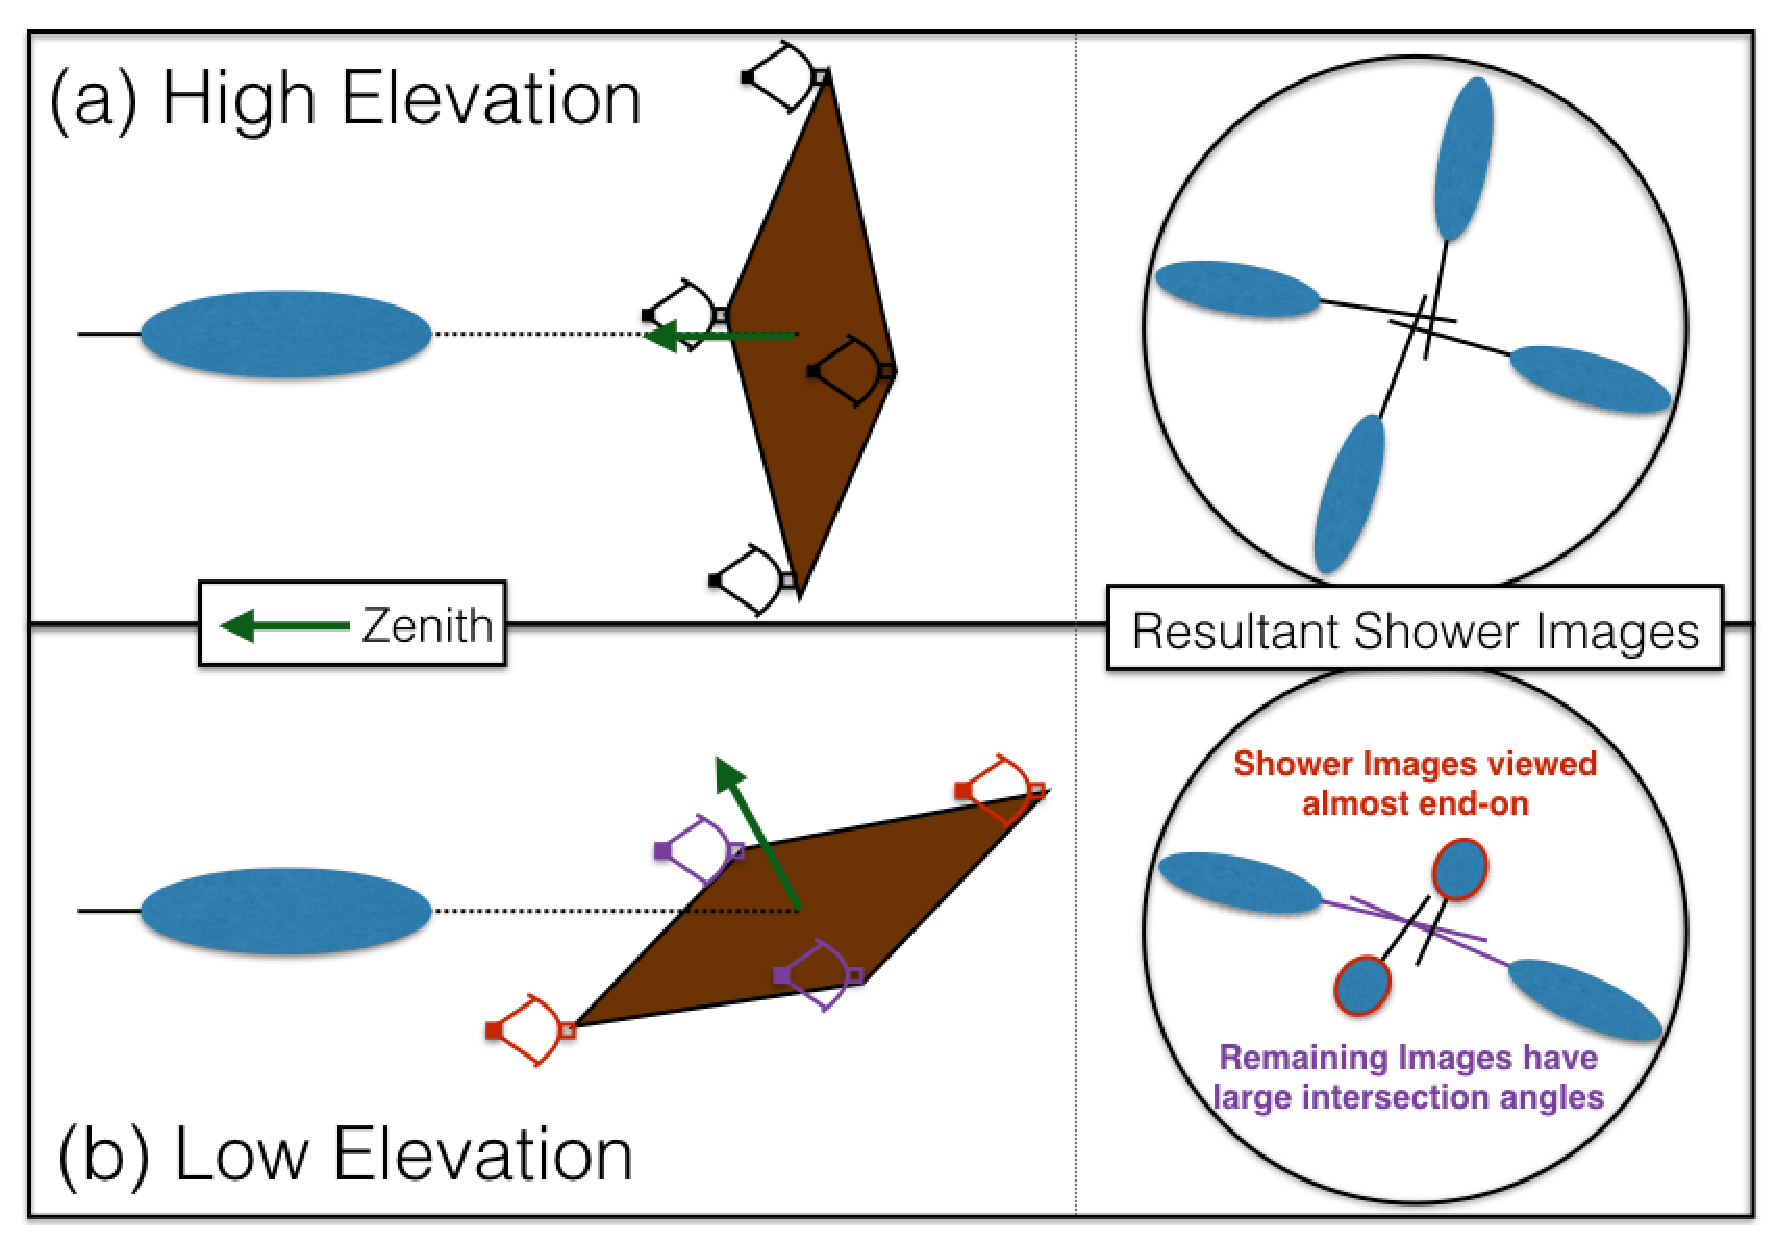
\includegraphics[width=0.75\textwidth]{images/high_elevation_vs_low_shower_images_cropped.eps}
        \caption[Shower Images at High and Low Elevations]{In Figure (a), high elevation showers produce long images in all four telescopes.  In Figure (b), lower elevation showers produce shortened images in two telescopes, and the remaining images form large angle intersection.}\label{fig:showerhighlowelev}
      \end{center}
    \end{figure}

    To better handle these near-parallel image axes at low elevations, the reconstructed position can be determined from more parameters than just the weighted image axes intersection points.
    From simulations, the distance between the center of the Hillas shower image and the true position can be calculated, where the angular distance between the two is the \disp{} parameter\cite{Senturk:2011}, shown in Figure \ref{fig:dispdiagram}.
    Then, this \disp{} parameter can be provided to a machine learning algorithm \cite{Beilicke2012NIM}, along with other image parameters like:
    \begin{description}
      \item[\textit{width}:] image angular width
      \item[\textit{length}:] image angular length
      \item[\textit{wol}:] $\frac{\textrm{width}}{\textrm{length}}$
      \item[\textit{size}:] total image dc
      \item[\textit{ntubes}:] number of pixels in the image
      \item[\textit{loss}:] fraction of image pixels at the edge of the camera
      \item[\textit{asym}:] distance between image center-of-dc and the pixel with the highest dc
      \item[\textit{tgrad}:] the slope of the linear time fit to the pixel arrival times
      \item[\textit{cross}:] angular distance between the image center and the reconstructed gamma-ray position
    \end{description}
  % list of training parameters: grep "AddVariable" $EVNDISPSYS/src/trainTMVAforAngularReconstruction.cpp
  % how variables are calculated: grep -P "fParGeo.+\=" $EVNDISPSYS/src/VImageParameterCalculation.cpp
  % asym: http://inspirehep.net/record/1395717/files/RdelosReyes.pdf
  % Once trained on these parameters, the machine learning algorithm can construct a boosted decision tree for determining any new image's \textit{disp}, which can then be used with the image axes intersections to improve the gamma-ray reconstructed positions.


    \begin{figure}[ht]
      \begin{center}
        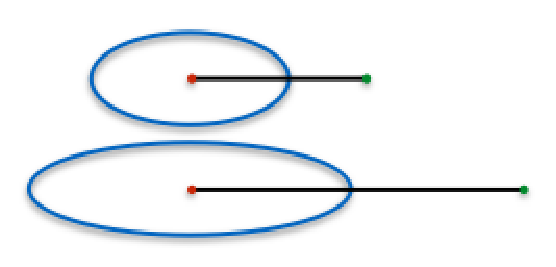
\includegraphics[width=0.5\textwidth]{images/disp_parameter_cropped.eps}
        \caption[Angular Reconstruction Disp]{The \disp{} parameter is the angular distance between the center (red dot) of a hillas image (blue oval) and the true sky position (green dot).  Generally, longer shower images have a larger \disp{} angle.}\label{fig:dispdiagram}
      \end{center}
    \end{figure}

    % https://veritas.sao.arizona.edu/wiki/index.php/BDT_Angular_reconstruction
    These parameters for thousands of simulated showers can then be used to train a boosted decision tree forest (BDT) that estimates the most probable \disp{} for a new shower's images.
    This most-probable \disp{} can then be used with the image axes intersection points to more accurately reconstruct the original gamma-ray point of origin.
    
    Once the training is complete, it is tested on a separate set of 17,000 simulated events, which are plotted in Figure \ref{fig:disptraining}.
    The x axis describes the true \disp{} value for each event, while the y axis describes the \disp{} value estimated by the BDT, with a black $x=y$ line marked, which represents a perfect 1:1 \disp{} reconstruction.
    As events fall on the $x=y$ line, it can be concluded that the BDTs are able to predict the correct \disp{} value for most images.

    % made from screenshot of last slide in Dropbox/Presentations/20160719_Group_Meeting.key
    \begin{figure}[ht]
      \begin{center}
        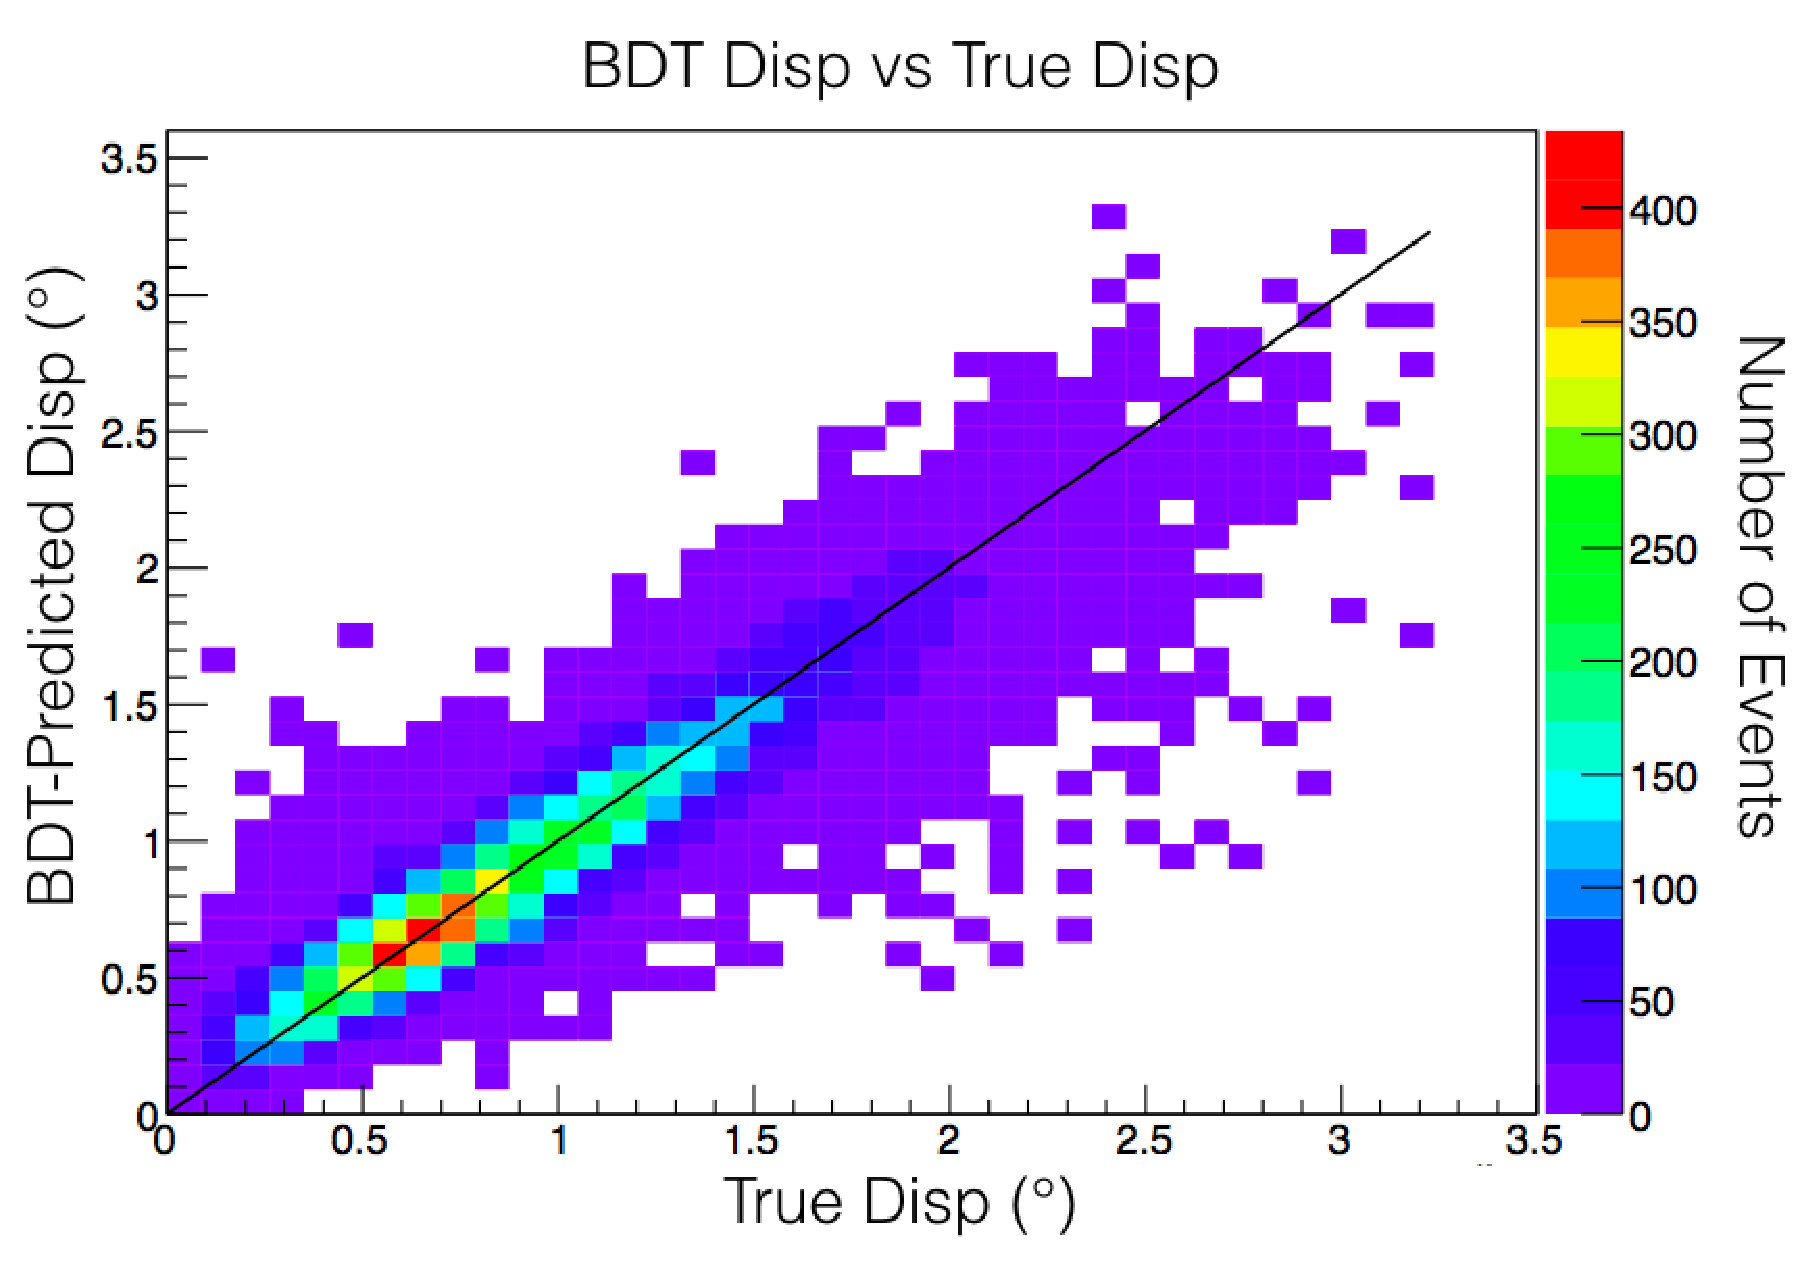
\includegraphics[width=0.85\textwidth]{images/disp_training.eps}
        \caption[Disp BDT Training]{The true \disp{} vs the BDT-predicted \disp{}, for \nicetilde17,000 gamma-ray event images in T1, from 500\GeV to 200\TeV.}\label{fig:disptraining}
      \end{center}
    \end{figure}

    The small improvement in the position reconstruction due to the \disp{} method can be seen in Figure \ref{fig:disp_event_offset}.
    With the Geometric (red) events, more are concentrated further from the point source, while with the Disp method, somewhat more are concentrated at the source itself.

    \begin{figure}[ht]
      \centering
      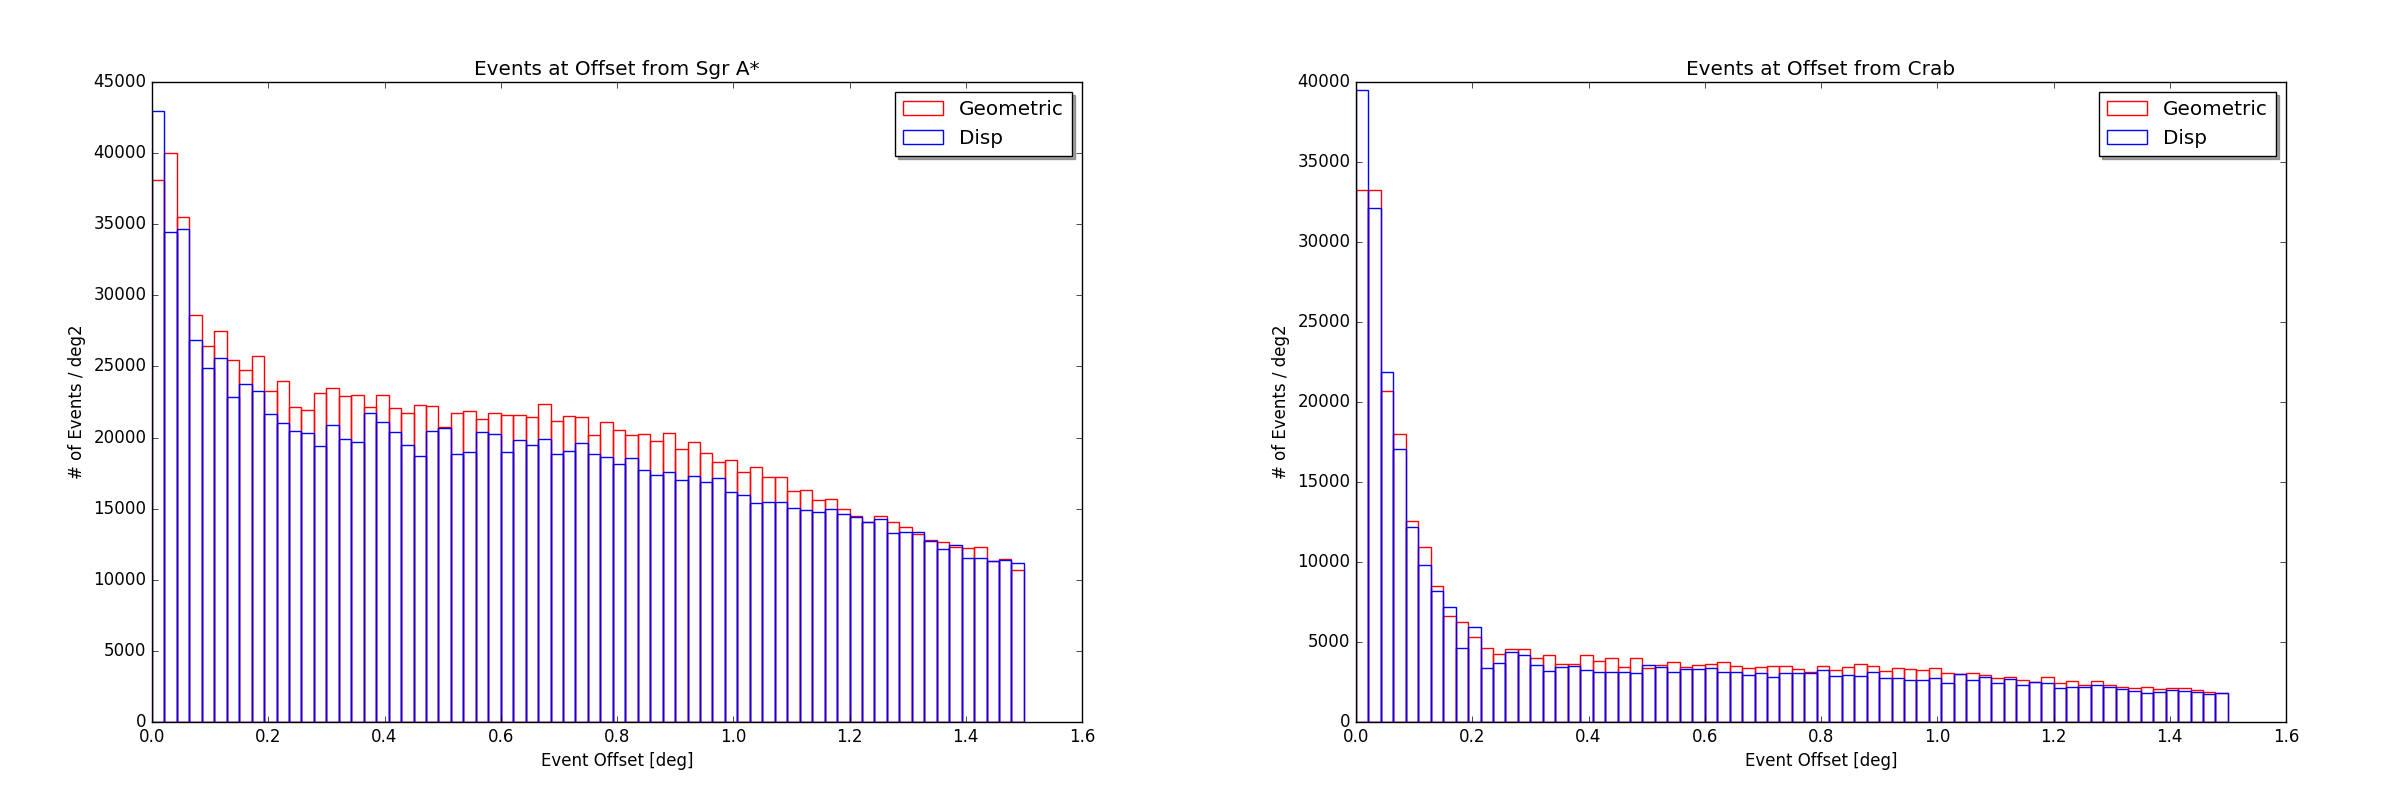
\includegraphics[width=\textwidth]{images/disp_event_offset_hists/disp_event_offset_hist.eps}
      \caption[DISP Offset Improvement]{
        The number of events per solid angle at different angular offsets from the Crab and the Galactic Center, with both Geometric and Disp reconstruction methods.
        The labels and legend in the plots should be bigger (rule of thumb is the same size as the general text of the document). 
        Would be great to put the mean and RMS on the plots, so you can quantify the differences.
        In the caption, point to left and right plot (or use sub-figures)?? -Orel)
      }
      \label{fig:disp_event_offset}
    \end{figure}

\section{Energy Reconstruction}\label{subsec:enrecon}
  To reconstruct the energy of each shower, a database of simulated showers is built.
  This database includes the width and length of the shower, how far away its core position is, how bright it was, as well as its reconstructed and true energy.
  By scanning through this database for showers that are similar to the one being constructed, the most similar-looking shower then indicates the true energy(is there any interpolation?? -Orel, ask gernot).

\section{FITS Conversion for Gammalib and CTOOLs}
  Once gamma rays have been reconstructed with event display, they must be converted to a FITS file format compatible with Gammalib and CTOOLS.
  This format consists of a FITS file with an event list table, containing each gamma ray, its energy, sky direction, and time.
  This also includes meta information about the event list like the telescope's pointing target and the start and end times of the event list.
  This FITS file can then be read into Gammalib and CTOOLS \cite{gammalibctools}.

  In addition to the event list, the instrument response functions (IRFs) must also be imported into Gammalib and CTOOLS.
  These IRFs consist of the effective areas, the point spread functions, the background models, and the energy dispersion.
  The effective area quantifies the total gamma-ray collection area of the observatory, needed for spectral measurements, and is described in subsection \ref{subsec:effarea}.
  The point spread function quantifies the distribution of true positions for a reconstructed position, needed for identifying point sources and extended spatial structures, and is described in subsection \ref{subsec:psf}.
  The background models measure the relative number of observed events in different parts of the camera, and their construction is described in subsection \ref{background_production}.
  The energy dispersion quantifies the distribution of true energies for a given reconstructed energy, and is discussed in subsection \ref{subsec:edisp}.

  Each of these IRFs vary in a parameter space with several dimensions, including event Energy, reconstructed distance from the camera center, telescope elevation and azimuth, night sky background noise, and the atmospheric density.
  In CTOOLS' default configuration, all IRFs are stored in a single directory of files, and each event list contains a filepath reference to indicate which volume of the parameter space it uses.
  Once each volume is loaded, individual events can then interpolate their specific effective area, psf, and energy dispersion (the backgrounds are utilized differently, as discussed in subsection \ref{background_production}).

  However, the galactic center is at an elevation of $\ang{30}$, much lower than most VERITAS observation targets.
  At this elevation, with its field of view of $\ang{3.5}$, the airmass column density ($g/cm^{2}$) is 20\% higher at the bottom of the camera than at the top.
  Add to this that during a single 30 minute observation, the elevation of the Galactic Center can change by several degrees, means the airmass in view of the camera may change rapidly, meaning the IRFs may become time dependent.

  To allow for the inclusion of this time dependence in the analysis, an alternate way of storing the IRFs was chosen, diagrammed in Figure \ref{fig:fits_scheme}.
  First, one observation (typically 20-30 minutes long) is broken up into \nicetilde8 minute chunks.
  Each chunk is then converted to an event list, and saved to a FITS file.
  In addition, the needed effective areas, psfs, and background models are also written to the same FITS file.
  As each event list covers a small region in time, the IRF tables only need to contain the dimensions of the parameter space that can change during one chunk, such as event energy and distance from camera center.

  \begin{figure}[ht]
    \centering
    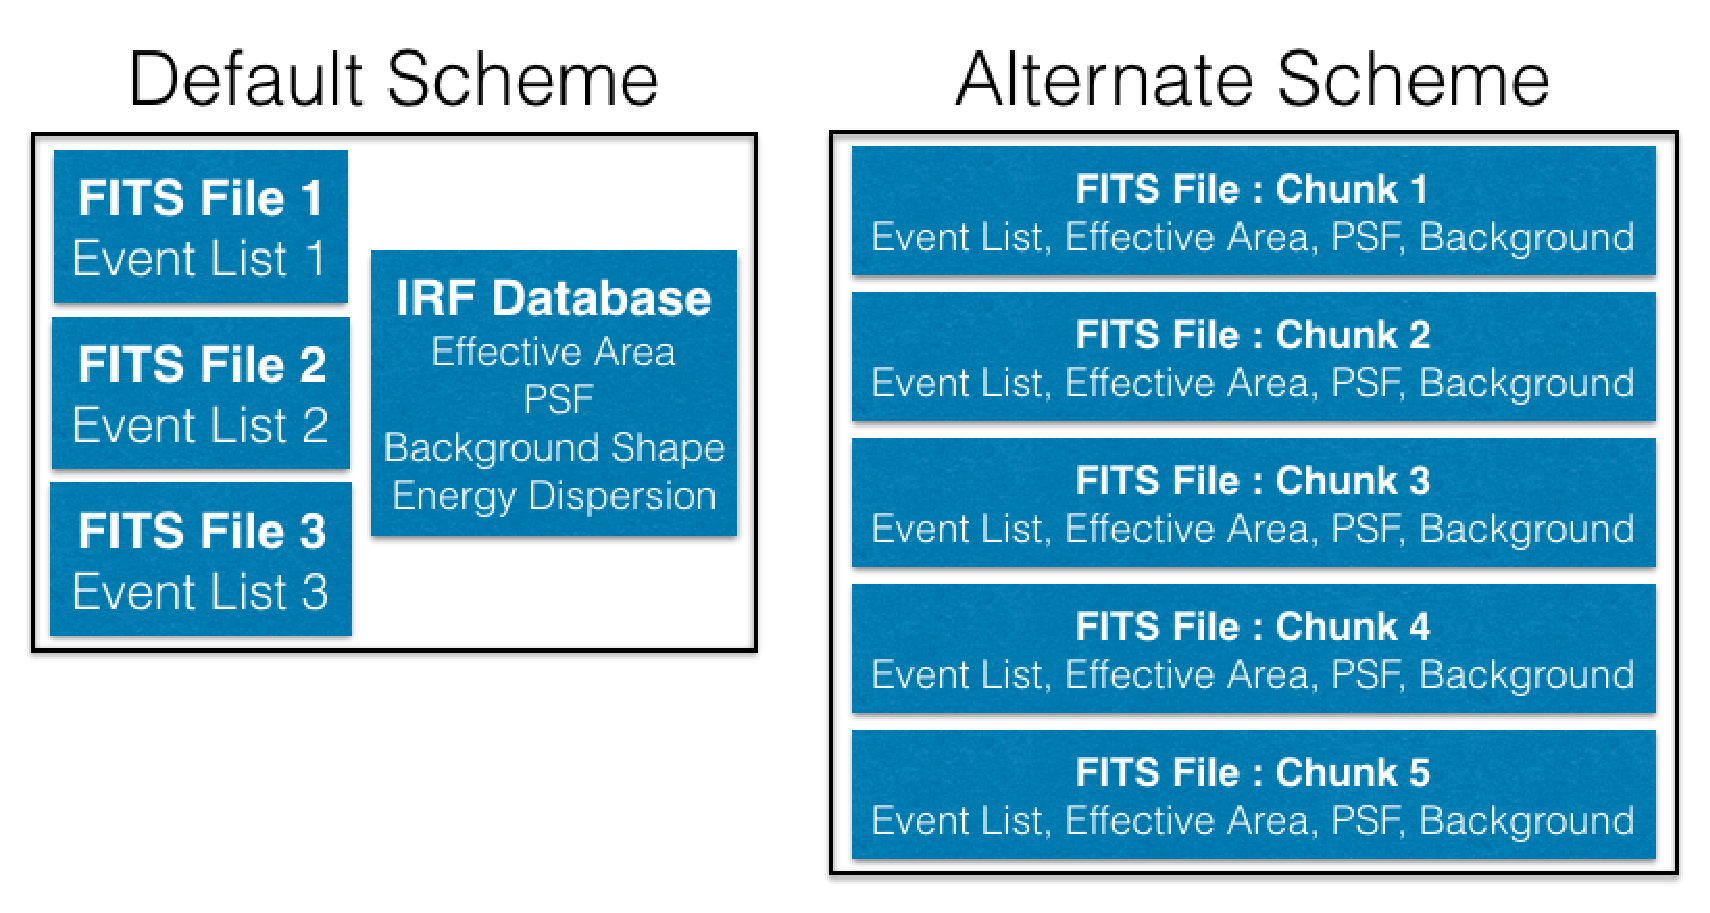
\includegraphics[width=0.75\textwidth]{images/FITS_diagrams_alternate_scheme.eps}
    \caption[FITS File Event Storage Schemes]
    {Fits file storage schema.}
    \label{fig:fits_scheme}
  \end{figure}

  The end result is that a 30 minute observation can be broken into several FITS files (called chunks), where each chunk file is independent of any outside references, contains all needed IRF information, and only takes up \nicetilde\SI{5}{MB} on disk.
  This makes it ideal for an analysis program to automatically download any needed data over an internet connection, as each chunk is tiny and has no outside dependencies.
  As gammalib and CTOOLS expect the default FITS file scheme, a python function was written to automatically load all event and IRF tables from a single fits file, and import this information into gammalib's GObservation class.

  There were minor issues with converting the IRFs that are noted in the following sections.


  \subsection{Effective Area}\label{subsec:effarea}
    % use effective area as a casual noun!
    % plot of effective area vs energy
    Effective area is the measure of how large an observatory's collection area is, determining how many gamma rays can be detected per unit time, solid angle, and energy.

    For each point in the parameter space, the effective areas are calculated with many Monte Carlo gamma ray simulations.
    This is done in the shower plane, the plane perpendicular to the line drawn between an observing source, and the center of the observatory.
    The effective area is then calculated via:
    $A=\pi R^2 \frac{N_{\text{survived}}}{N_{\text{simulated}}}$
    where R is the radius of the area within which simulated showers are directed to fall, $N_{\text{simulated}}$ is the number of showers that were initially simulated into the area, and $N_{\text{survived}}$ is the number of simulated showers that pass all cuts.
    This effective area is thus a measure of how much detection area the observatory would have if it had a 100\% detection efficiency, which can then be used in calculating a source's flux.
    In Figure \ref{fig:effarea_paramspace}, it can be seen how the effective area peaks to \nicetilde{}\SI{3e5}{m${}^2$} for \SI{3}{\TeV} events at the camera center.

    \begin{figure}[ht]
      \centering
      \includegraphics[width=0.85\textwidth]{images/effarea_plots/effarea_space.eps}
      \caption[Effective Area Parameter Space]{
        Effective areas at different points in the Energy and Camera Offset parameter space for run 78128.
        Some event positions within the parameter space are shown as black dots.
      }
      \label{fig:effarea_paramspace}
    \end{figure}

    For the test analyses of the Crab and the Galactic Center Point Source, the effective areas of all events are shown in Figure \ref{fig:effarea_usage}.

    \begin{figure}[ht]
      \centering
      \includegraphics[width=0.85\textwidth]{images/effarea_plots/effarea_events.eps}
      \caption[Effective Areas Used]
      {Effective areas used by events in each analysis.}
      \label{fig:effarea_usage}
    \end{figure}

    \subsection{Point Spread Function}\label{subsec:psf}

    When reconstructing the source position of each gamma ray, it is necessary to know the uncertainty of the position.
    Primarily, errors in the position come from the randomness of shower images.
    The same gamma ray may develop into a different shower (with different particles early in the shower gaining different amounts of energy or scattering at different angles), or different shower cherenkov photons may be absorbed by the atmosphere, or reflected by the mirrors, or converted into PMT photoelectrons.
    In the image and position reconstruction, this means that an initial gamma ray from some initial position can develop into a distribution of camera images, and vice versa, that a single shower image can come from a distribution of gamma ray positions.

    This distribution of reconstructed positions, called the point spread function (psf), primarily affects the shape of gamma-ray emission structures in the sky.
    A singular point source, nominally shaped by a dirac function, is instead distributed out according to the psf.
    When searching for an extended source, like a dark matter halo, understanding the distribution of reconstructed positions is important.
    A large psf on all events, for instance, will artificially expand a dark matter halo.

    For VERITAS, the psf is estimated by simulating many gamma rays, then measuring the distribution of true positions for each reconstructed position.
    With VERITAS and Event Display, a gaussian was chosen to fit the psf distribution.
    For CTOOLS however, the distribution of events are instead fitted with a King function \cite{king1962} (see eqn \ref{eqn:king}), as Fermi \cite{fermipsf} has found gamma ray psfs tend to have longer tails than a Gaussian, which the king function better handles.
    The radially-normalized king probability density function is defined as

    \begin{equation} \label{eqn:king}
    \text{psf}_{king}(r) = \frac{1}{2 \pi \sigma^{2} } \left( 1 - \frac{1}{\gamma} \right) \left( 1 + \frac{ r^{2} }{ 2 \gamma \sigma^{2} } \right)^{-\gamma}
    \end{equation},

    where $r$ is the angular distance from the reconstructed position, $\sigma$ is similar to the width of a gaussian, and $\gamma$ governs how long the tails are.
    A king function fitting algorithm was added to Event Display, that fits the $\gamma$ and $\sigma$ parameters to a set of simulated gamma rays.
    This leads to good fits over almost all of the parameter space.
    In Figure \ref{fig:psf_paramspace}, the psf is shown for one Galactic Center run.
    In it, one can see how the psf containment radius changes vs reconstructed energy and offset from the camera's center.
    Other runs, which have different elevations, azimuths and NSB noise levels will have different values at each point in the energy/offset parameter space.

    % plot of psfs from chunkplot
    \begin{figure}[ht]
      \centering
      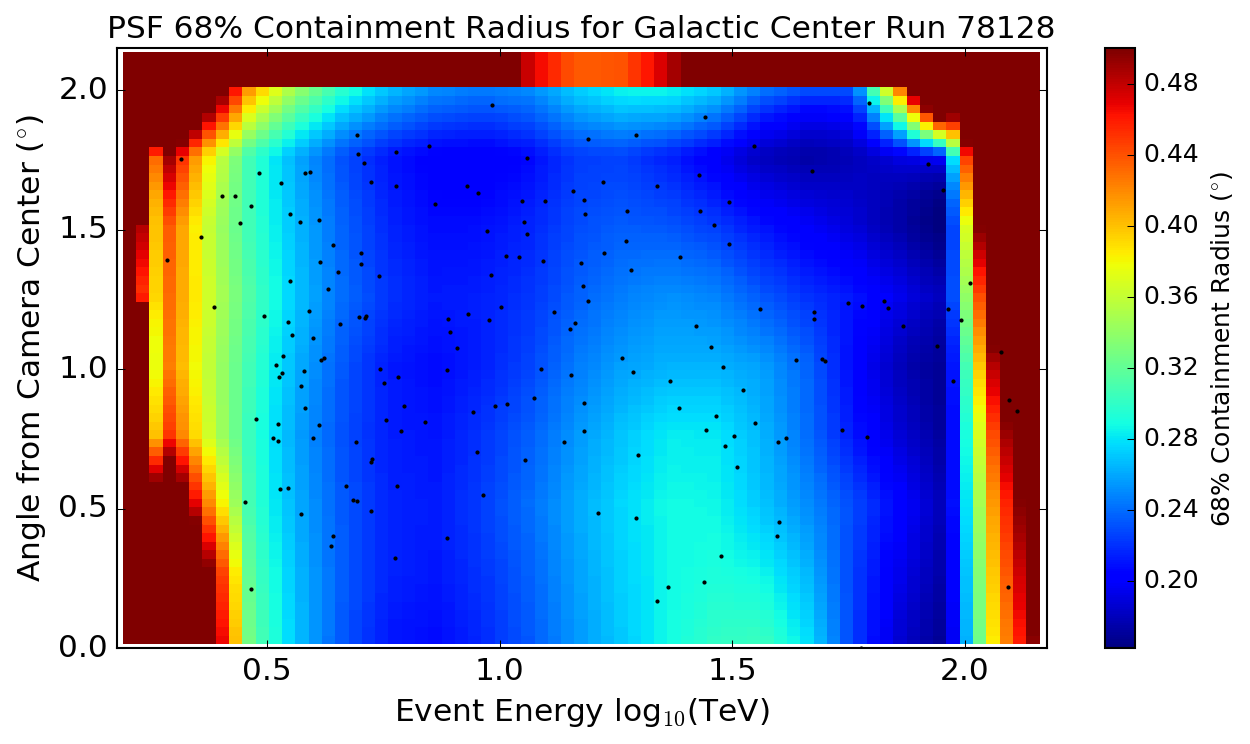
\includegraphics[width=\textwidth]{images/psf_king_plots/psf_parameter_space.eps}
      \caption[PSF Parameter Space]{
        The 68\% containment radius for the Energy/Offset parameter space for Galactic Center run 78128. 
        The green points show a subset of the event positions from that run in the parameter space.
      }
      \label{fig:psf_paramspace}
    \end{figure}

    For the Galactic Center and the Crab analyses, the distribution of 68\% containment radii for all events is shown in Figure \ref{fig:gc_psf_hist}.

    \begin{figure}[ht]
      \centering
      \includegraphics[width=0.85\textwidth]{images/psf_gc_eventhist/eventpsf.eps}
      \caption[Crab and Galactic Center Event PSFs]{
        The 68\% containment radius for all Galactic Center and Crab events used in this analysis.
      }
      \label{fig:gc_psf_hist}
    \end{figure}

  \subsection{Background Models}\label{background_production}
    A background model is a 3 dimensional function in camera X (in angle, parallel to azimuth), camera Y (in angle, parallel to elevation), and energy.
    The function predicts the number of observed events in the camera, per unit solid angle, unit time, and unit energy.
    This is used to quantify how many counts are expected when observing a gamma-ray-dark sky position, which estimates how many background proton events are being detected at different energies and in different parts of the camera.
    Understanding the background shape of the camera is crucial for properly studying extended sources, like dark matter halos, which may extend several degrees from the galactic center.
    Improperly estimating background models can create fake structures in an astrophysical target.
    Background models with more than three dimensions are also possible, but require many more simulations, and are beyond the scope of this thesis.

    To produce a background model, gamma-like events from 'dark' obsevations (areas of the sky with no gamma-ray sources) are binned in camera coordinates and energy.
    The details of the selected dark observations are detailed further in \ref{veritasdata}.
    The energy bins are determined by expanding outwards (in log${}_{10}(\TeV{})$ space) from the median energy of all events, until each energy bin has at least 100 events per \degreesquared{}.
    Any energy bins at the upper or lower edges that have less than 100 events per \degreesquared{} are absorbed into the neighboring energy bin.
    This 100 events per \degreesquared{} was chosen because in test plots, this theshold provided enough events for a smooth Camera X/Y 2D histograms at a useful resolution (\nicetilde60 bins across one dimension of the field of view) which form the background models.
    In these energy bins, events are then binned radially, which is then used to fit an interpolation function (see Figure \ref{fig:background_radial}).
    This interpolated function is normalized so that its volume is equal to the initial number of events. 

    These energy-bin pdfs can then be interpolated linearly in log${}_{10}(\TeV{})$ space, to get the radial distribution of events at various energies.

    \begin{figure}[ht]
      \centering
      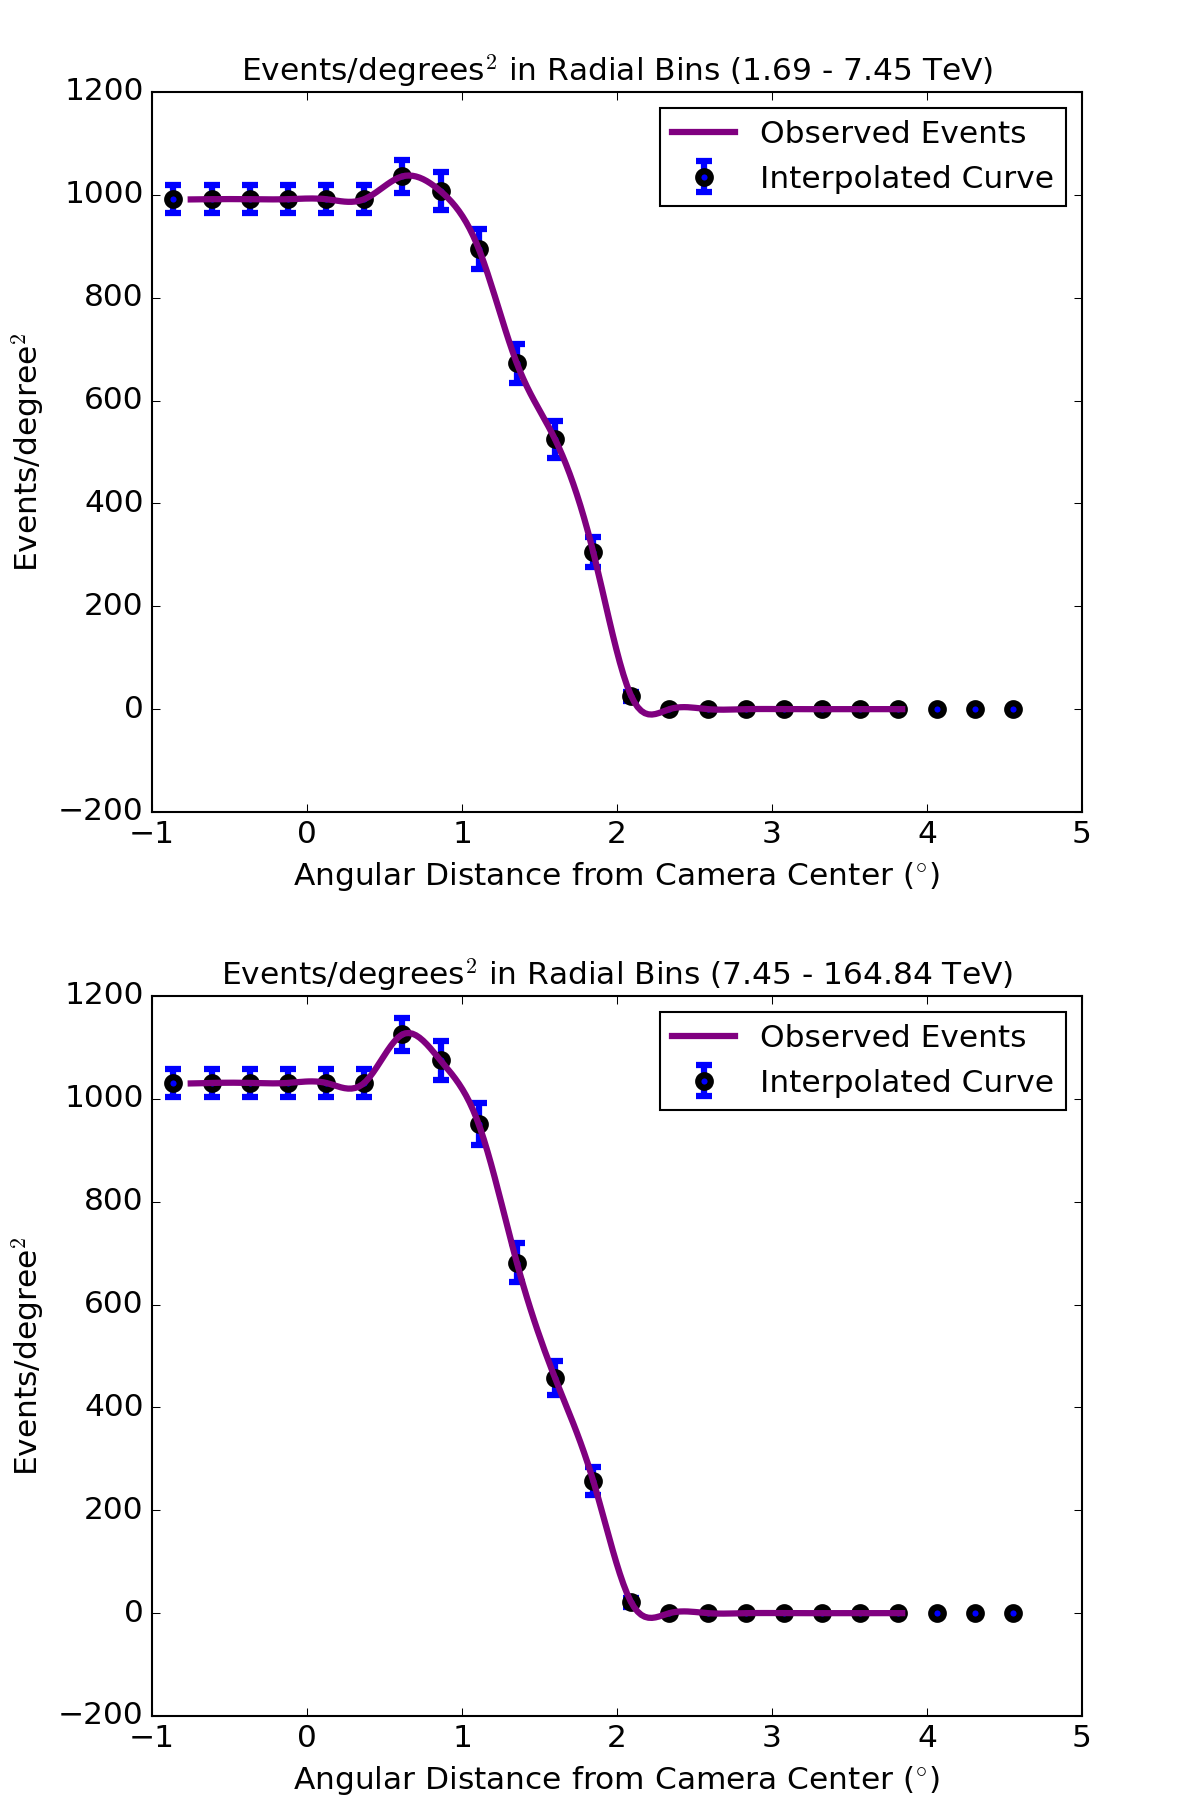
\includegraphics[width=0.7\textwidth]{images/ctools_background/radial_profiles.eps}
      \caption[CTOOLS Radial Background Profiles]{
        Radial bin profiles for the V5 background's two large-scale energy bins.
        The blue points are the counts per bin area, while the purple line is the interpolation with a spline interpolator of order 3 (see scipy.interpolate.interp1d())
        }
      \label{fig:background_radial}
    \end{figure}


    Then, all events are divided up into \nicetilde30 finer energy bins as shown in Figure \ref{fig:background_profile}, and each bin's counts are multiplied by the interpolated radial pdf at that energy, which is then written to a two-dimensional array of camera x/y bins.
    2D bin values are then divided by the solid angle of the bin (in sr), the energy width of the bin (in MeV), and the total obseration time (in seconds).

    (For the above 2-3 paragraphs: I really have trouble following what is done exactly and I think there is no need to go into these details. This looks like a description of the code instead of the physics/analysis. --Orel??)

    \begin{figure}[ht]
      \centering
      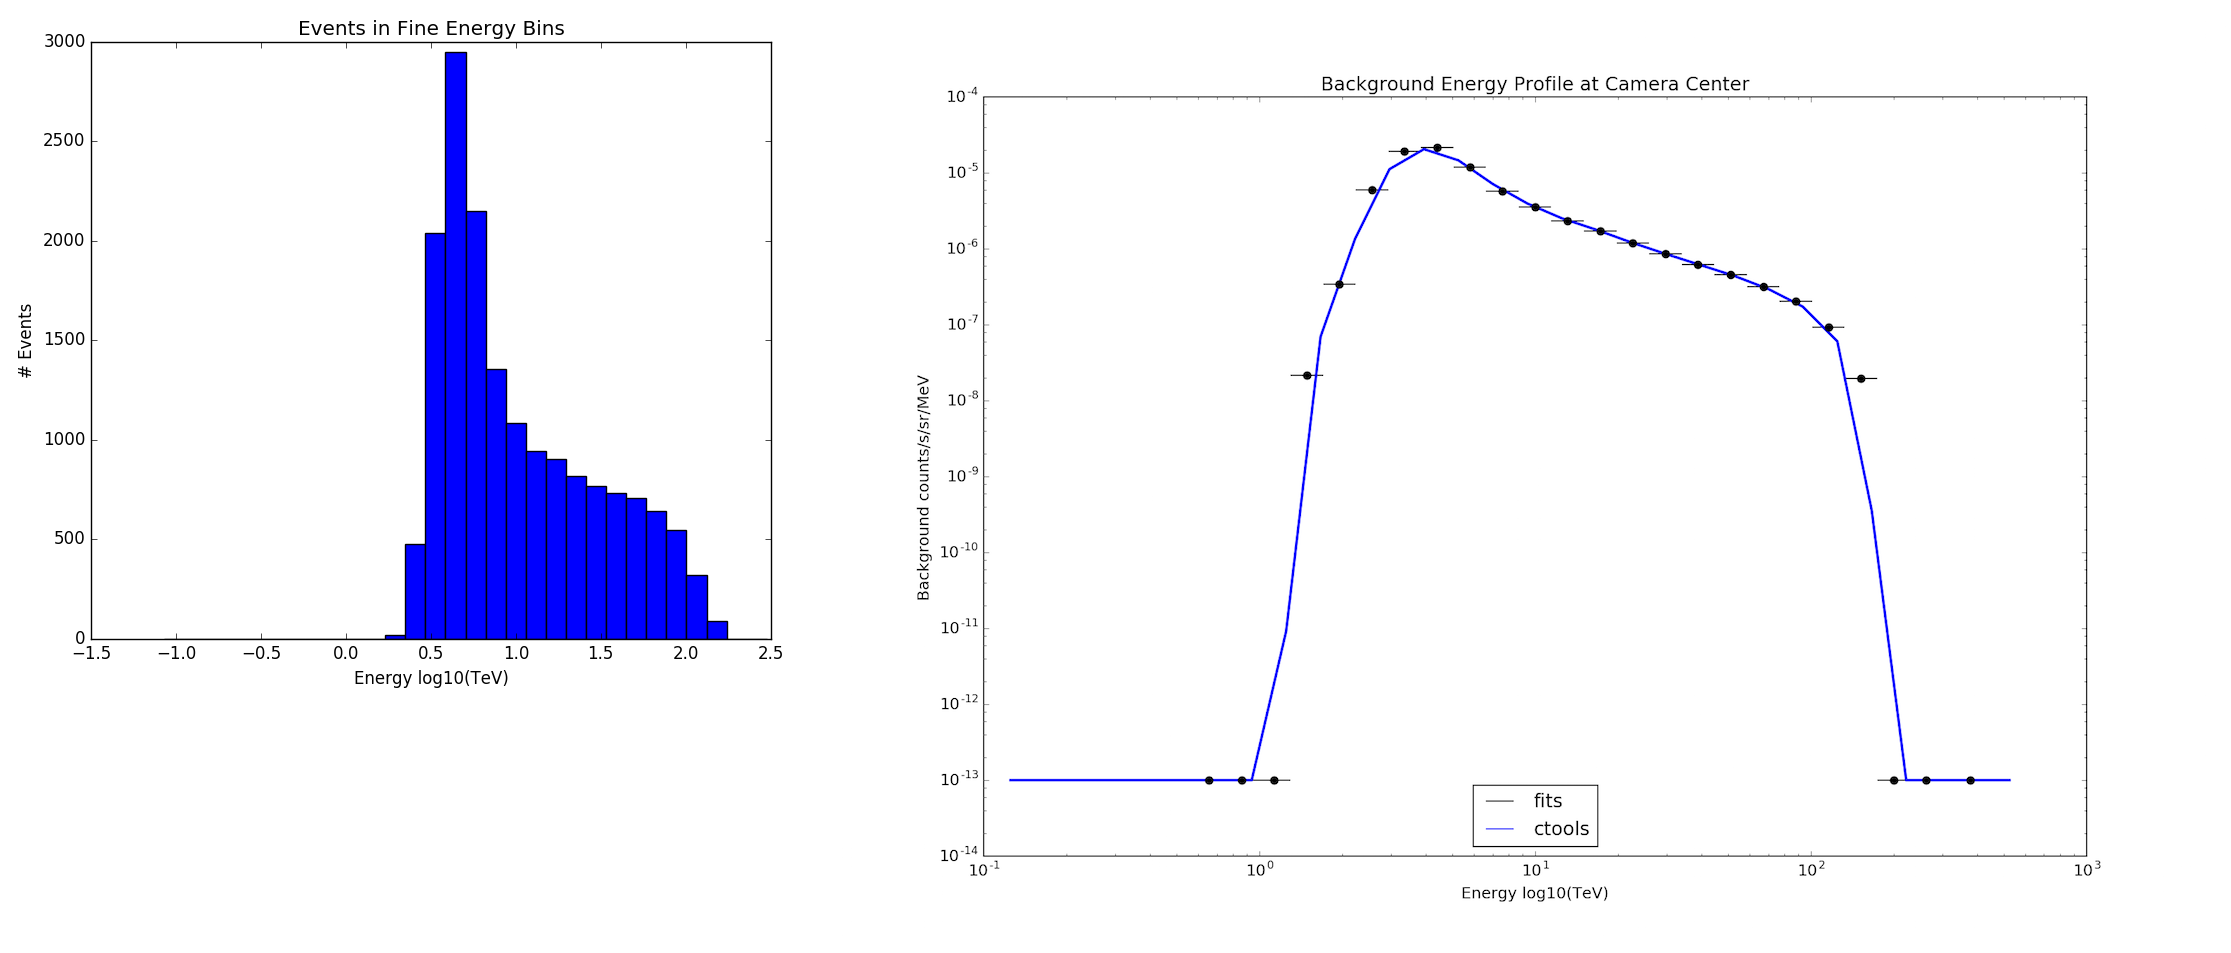
\includegraphics[width=0.7\textwidth]{images/ctools_background/background_construction.eps}
      \caption[CTOOLS Background Fine Energy Bins]{
        The V5 Background's fine-energy bins.
        The top plot shows the number of events in each fine-energy bin.
        The bottom plot shows the CTOOLS background values.
        The black lines show the fits background value and energy bin width saved to the background file, while the blue line shows the background value after CTOOLS loads and interpolates those fits background values.
      }
      \label{fig:background_profile}
    \end{figure}

    The background is used in the likelihood analysis as a model with two free parameters, a simple multiplicative normalization factor, and a power law spectral index.
    This lets the likelihood engine scale each run's background model up or down to best fit the events, so the background's absolute value is less important than the relative values in different parts of the camera.

  \subsection{Energy Dispersion}\label{subsec:edisp}
    As events are reconstructed imperfectly, it is important to understand what the distribution of true energies are for a given reconstructed energy.
    In an analysis with CTOOLS, this is quantified by an energy migration matrix $E_{i,j}$, where $i$ denotes the $i^{\text{th}}$ reconstructed energy bin, and $j$ denotes the $j^{\text{th}}$ true energy bin.
    For true energy $j$, the distribution of reconstructed energies $f_{\text{reco}}$ is,

    \begin{equation}
      \label{eqn:edispreco}
      f_{\text{reco}}(j)=\frac{E_{i,j}}{ \sum_{i}E_{i,j} }
    \end{equation}

    for reconstructed energy $i$, the distribution of true energies $f_{\text{true}}$ is,

    \begin{equation}
      \label{eqn:edisptrue}
      f_{\text{true}}(i)=\frac{E_{i,j}}{ \sum_{j}E_{i,j} }
    \end{equation}

    By unfolding these distributions from the reconstructed energies, two primary analysis effects are accounted for.
    The first is that the reconstruction software introduces biases in the event energy, meaning on average, an event at a given true energy is reconstructed at a higher or lower energy.
    The second effect that is accounted for is the dispersion in the reconstructed energies.
    Multiple simulations of the same energy event will result in a distribution of reconstructed energies.
    This has the effect of smearing out events in each energy bin of a spectra.
    In astrophysical spectra, which often follow an exponential curve, lower energy bins tend to have more events than the next highest energy bin, so smearing out the lower-energy bin contributes more to the higher-energy bin than the higher-energy bin contributes to the lower-energy bin.
    This has the effect that, when not accounted for, energy dispersion will harden observed astrophysical source spectra.
    In Figure \ref{fig:migmatrix}, a migration matrix is shown.

    \begin{figure}[ht]
      \centering
      \includegraphics[width=\textwidth]{images/edisp_plots/edisp.eps}
      \caption[Energy Migration Matrix]{
        An energy migration matrix used with Galactic Center run 82288.
        The reconstructed energy is on the x axis, and the true energy is on the y axis.
        The z (color) axis (why does the z axis have units of 1/s*MeV??) denotes the number of simulated events that passed all cuts.
      }
      \label{fig:migmatrix}
    \end{figure}

\section{Camera Studies}
  The objective of this thesis is to put upper limits on the existance of an extended, faint gamma-ray emission region.
  In order to better understand the effects that impact the VERITAS camera behavior in reconstruction software, several studies were performed.

  \subsection{Background Structure at the Low Energy Threshold}
    During the production of the initial low elevation backgrounds, some new effects were noted.
    First, a series of gamma-like events were selected from observations with no known gamma-ray sources.
    These events were then divided into equal-statistics energy bins.
    For each equal-statistic energy bin, all the contained events were binned in camera X and Y.

    For a set of high-elevation observations, these backgrounds are shown in Figure \ref{fig:back_highelev}.
    It can be seen that all events are divided up into 3 equal-statistics energy bins in Figure \ref{fig:back_highelev}.A.
    Each energy bin is then binned in camera X and Y in Figure \ref{fig:back_highelev} B, C, and D.
    At these high elevations, the distribution of events in each energy bin is radially symmetric about the camera center.
    This happens because gamma ray's point of origin and its shower image in the camera are usually several tenths of a degree away from each other.
    In addition, the atmospheric mass-depth is similar in all parts of the camera.
    However, structures start to break the radial symmetry aat low energies and elevations.
    The cause of these structures is explored in the next section, \ref{subsubsec:diffusesims}.

    \begin{figure}[ht]
      \begin{center}
        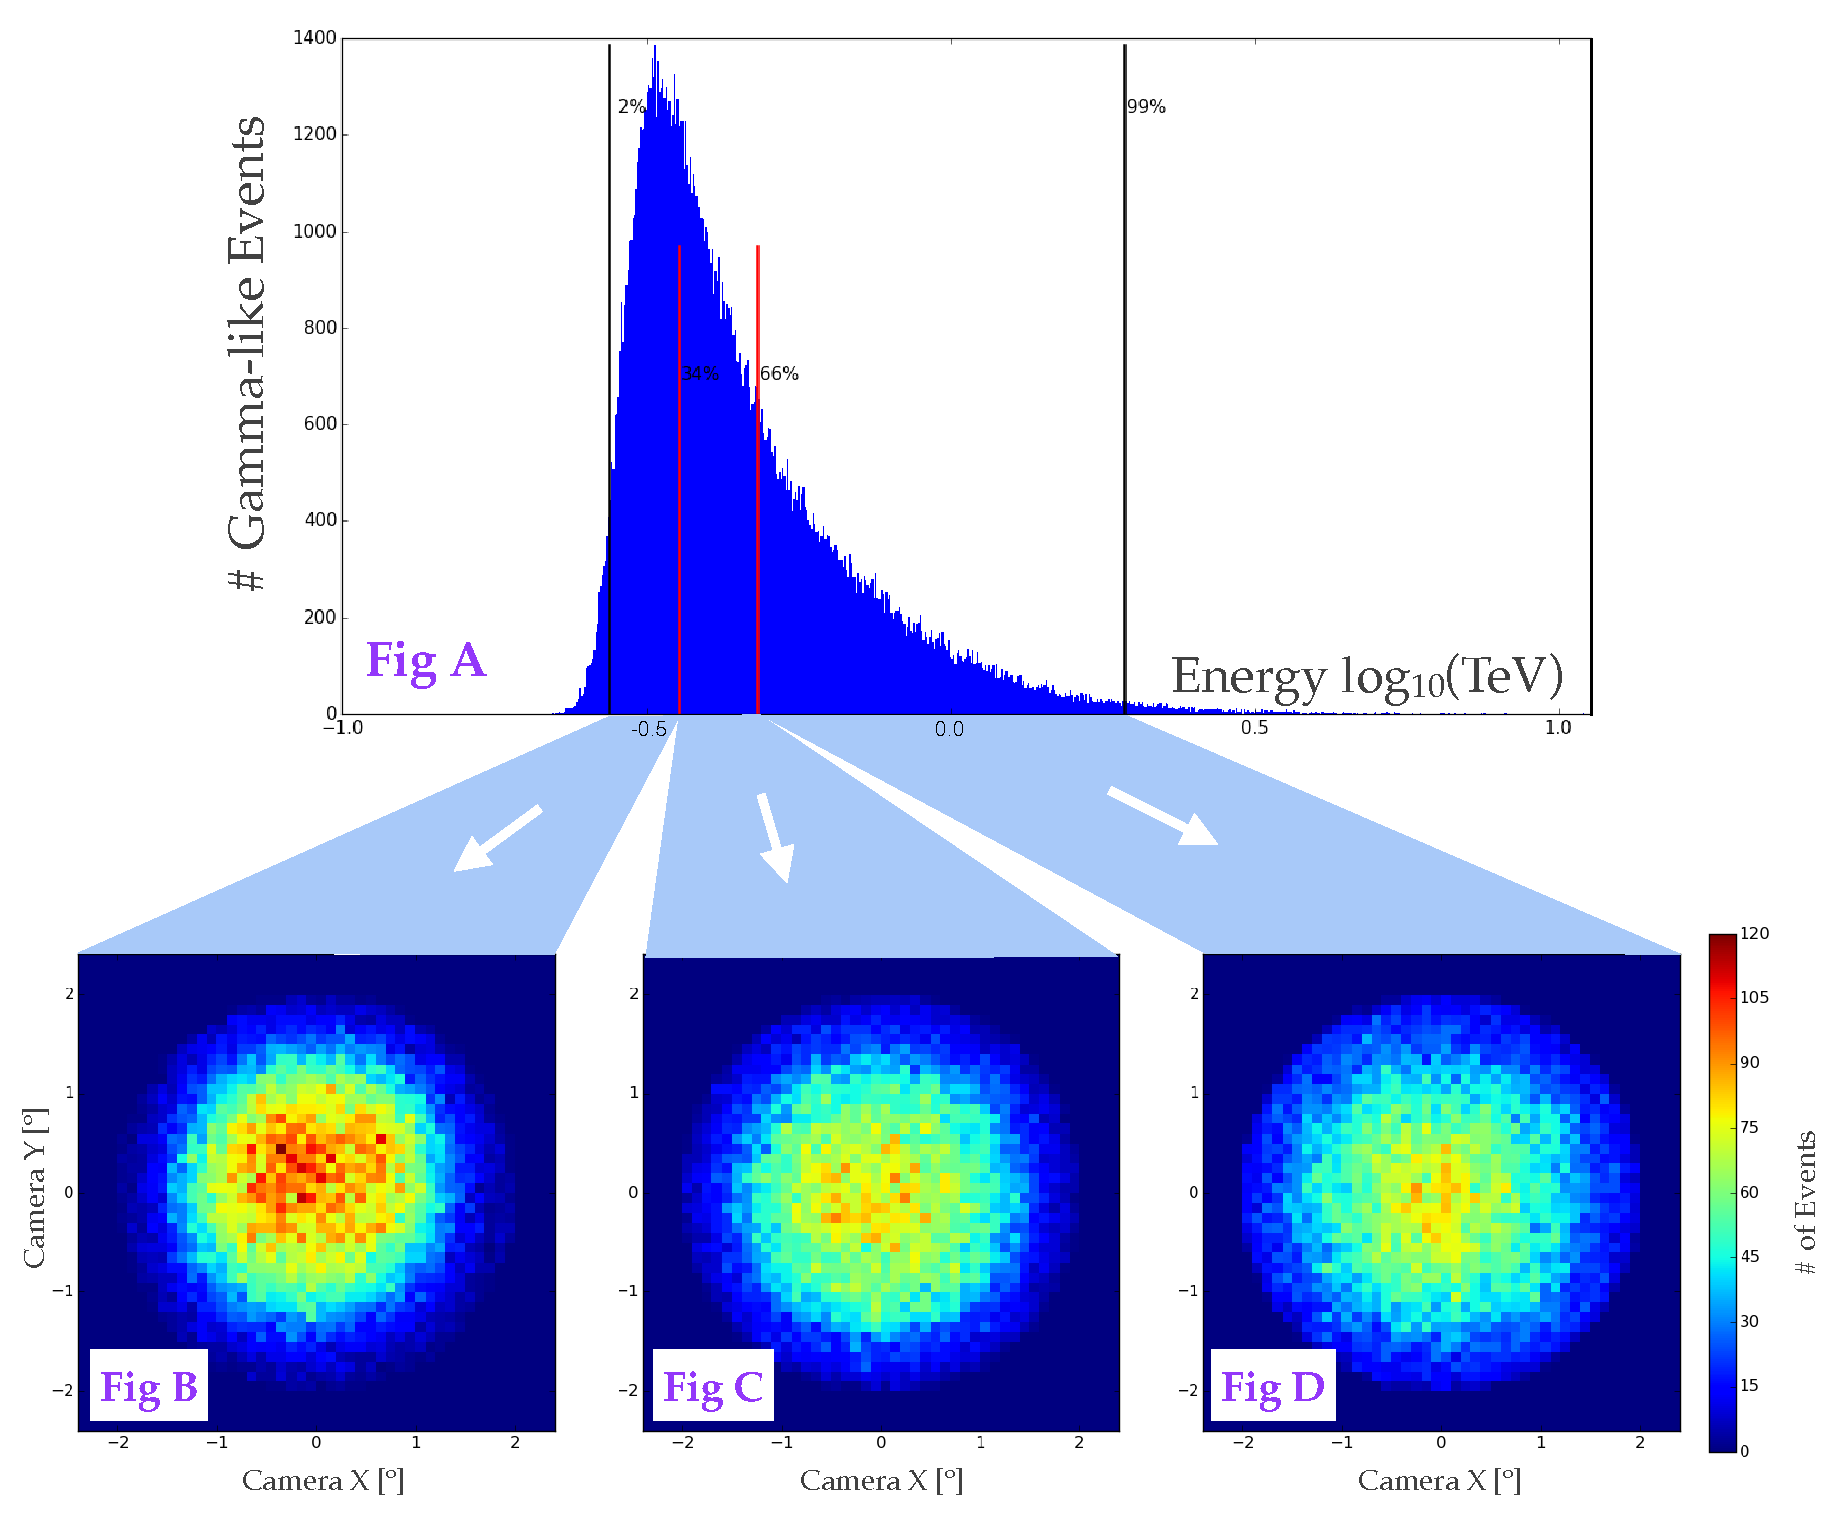
\includegraphics[width=\textwidth]{images/ctools/backgrounds_highelev.eps}
        \caption[FITS Background at 50\degree Elevation]{Gamma-like Events from 52 observations (approximately \nicetilde20 hours) of M82, between 50\degree  and 52\degree  elevations.  Events in Figure A are divided into 3 equal-statistics energy bins, and binned in Camera Coordinates in Figures B, C, and D. (change axes labels to only use Camera X and Y to be consistant with paragraph text --Orel??)}\label{fig:back_highelev}
      \end{center}
    \end{figure}

    In Figure \ref{fig:back_lowelev29} and Figure \ref{fig:back_lowelev26}, the same plots are constructed for a set of low-elevation ($ \nicetilde \ang{29} $ and $ \nicetilde \ang{26} $ respectivly) observations, using Galactic Center Off observations (reference these off observations to the apropriate section elsewhere??).
    These are again divided in to equal-statistic energy bins, and then each energy bin is binned in camera coordinates.
    It can be seen that in different energy bins, the background possesses different shapes.

    \begin{figure}[ht]
      \begin{center}
        \includegraphics[width=\textwidth]{images/ctools/backgrounds_lowelev29.eps}
        \caption[CTOOLS Background at 29\degree Elevation]{15 Sagittarius A* Off runs (\nicetilde7.5 observation hours), between elevations $ \ang{27.5} $ and $ \ang{30} $.  Events are divided into 6 equal-statistics energy bins, of which four are binned in Camera Coordinates in Figures B, C, D, and E.}\label{fig:back_lowelev29}
      \end{center}
    \end{figure}

    \begin{figure}[ht]
      \begin{center}
        \includegraphics[width=\textwidth]{images/ctools/backgrounds_lowelev26.eps}
        \caption[CTOOLS Background at 26\degree Elevation]{10 Sagittarius A* Off runs (\nicetilde5 observation hours), between elevations $ \ang{24} $ and $ \ang{27.5} $. }\label{fig:back_lowelev26}
      \end{center}
    \end{figure}
  
  After further studies, it was found that these structures depend on both the reconstructed energy and pointing elevation, and appears observations at distinct Right Ascension and Declinations.
  
  \begin{figure}[ht]
    \centering
    \includegraphics[height=\textheight]{images/background_vs_elevation/background_vs_elevation_srccrab.eps}
    \caption[Background Vs Elevation Crab]
    {\small 
      Plots of Crab observations.
      Top: Skymap of all events.  Middle: Histogram of all events in energy.  Bottom: Skymap of events from \SI{1.5}{\TeV}-\SI{3.25}{\TeV}.  
      In the bottom plot, events from \SI{1.5}{\TeV}-\SI{3.25}{\TeV} are concentrated in the top half of the camera (before being rotated to galactic (l,b) coordinates), due to the air column density ($g/cm^2$) being \nicetilde20\% smaller at the top of the camera.
    }
    \label{fig:bkgvsel_crab}
  \end{figure}

  \begin{figure}[ht]
    \centering
    \includegraphics[height=\textheight]{images/background_vs_elevation/background_vs_elevation_srcsgra.eps}
    \caption[Background Vs Elevation Sgr A*]
    {\small 
      Plots of Sgr A* observations.
      Top: Skymap of all events.  Middle: Histogram of all events in energy.  Bottom: Skymap of events from \SI{1.5}{\TeV}-\SI{3.25}{\TeV}.  
      In the bottom plot, events from \SI{1.5}{\TeV}-\SI{3.25}{\TeV} are concentrated in the top half of the camera (before being rotated to galactic (l,b) coordinates), due to the air column density ($g/cm^2$) being \nicetilde20\% smaller at the top of the camera.
    }
    \label{fig:bkgvsel_sgra}
  \end{figure}
  
  

  \subsubsection{Diffuse Simulations}\label{subsubsec:diffusesims}
    To rule out any software causes, diffuse simulations were performed at similar energies and elevations.
    These consisted of 50,000 gamma rays at each of 1.4, 1.6, 2, and \SI{5}{\TeV}.
    The telescopes were fixed to an azimuth/elevation of (193\degree,28\degree).
    The events themselves were distributed in a diffuse disk of radius 2.5\degree.
    After having their energy reconstructed, any events falling outside a simple mean-scaled-width cut of -2.0 to 0.5 were removed, which removes many of the showers that appear proton-like, approximating a gamma-hadron cut.
    These are then binned in camera coordinates in Figure \ref{fig:back_simdiffuse}.

    \begin{figure}[ht]
      \centering
      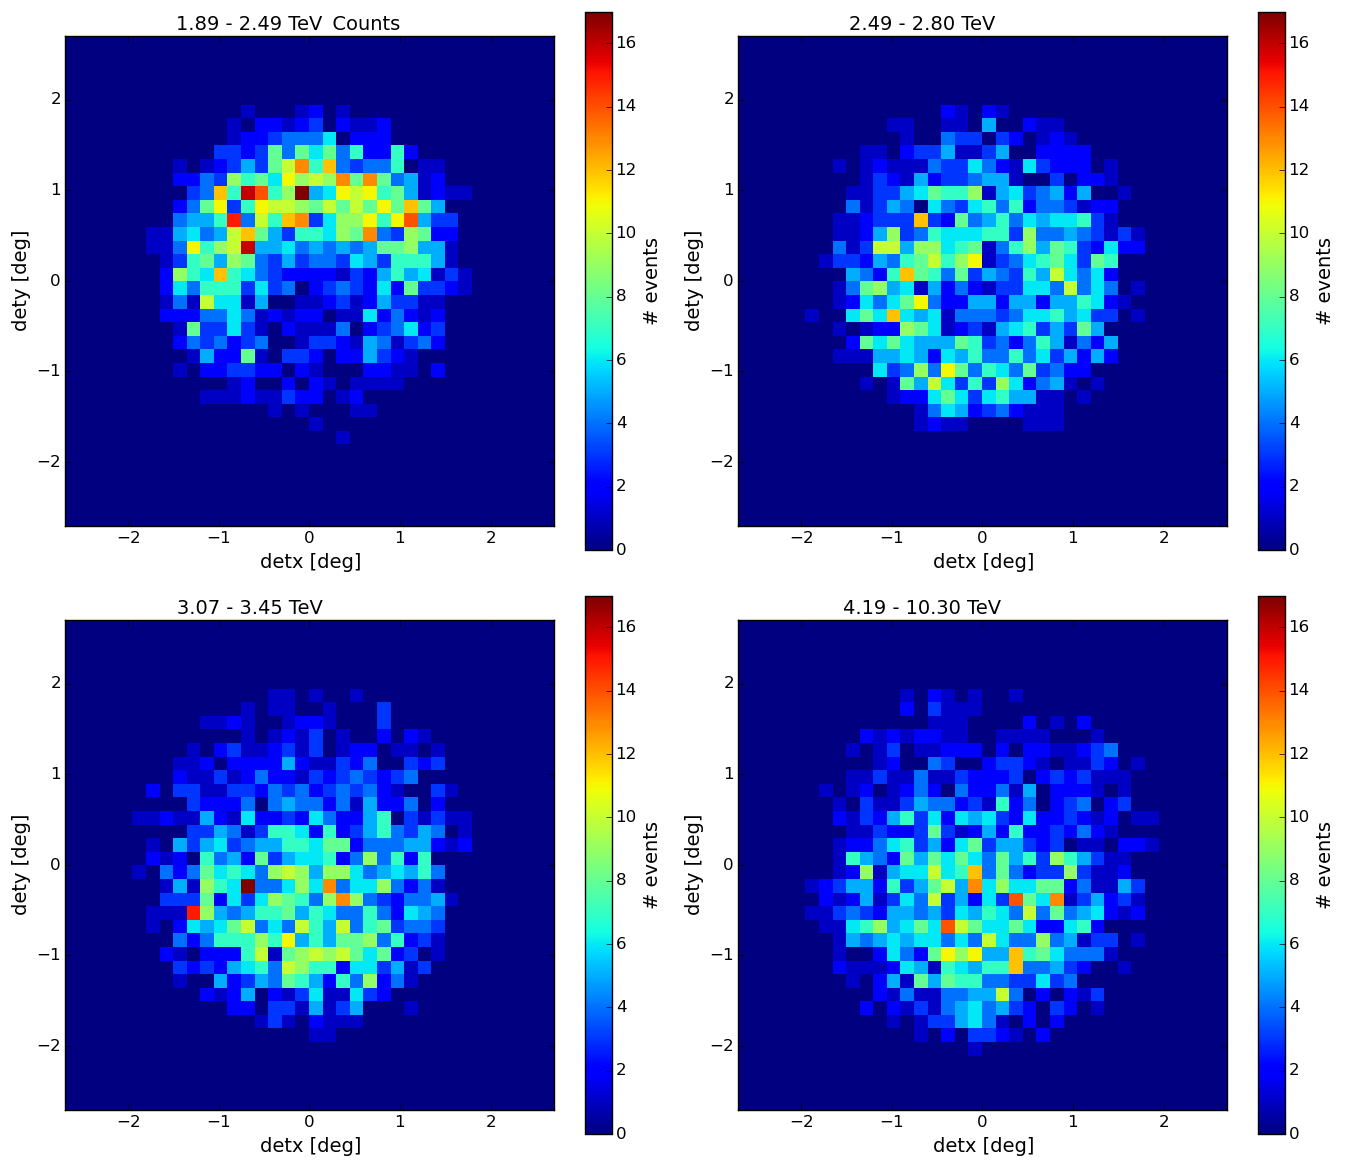
\includegraphics[width=\textwidth]{images/backgrounds_diffuse_vs_data/diffuse_sims.eps}
      \caption[Diffuse Simulated Backgrounds]{
        Diffuse simulated gamma-like events in the camera coordinate system at a 28\degree elevation, at 4 different energies.
      }
      \label{fig:back_simdiffuse}
    \end{figure}

    One can see that the ring and crescent structures persist in these diffuse simulations, implying these are physical effects of the atmosphere and camera, rather than a problem with the reconstruction software.
    (But what is the effect? I remember Gernot mentioning something about an edge effect? You should explain it here. --Orel??)

    This striking effect can be seen in Galactic Center data between certain energy ranges.
    As the plots are in galactic (l,b) coordinates, and there is a time rotation due to the Earth spinning on its axis, the crescent shapes are still present, albiet smeared around the 4 wobble targets.

    plot of events around galactic center (all energies vs @2 \TeV ) !??
    
    These structures, and their strong dependency on both the energy and elevation of the telescopes may be a large factor in why the low-energy threshold regime of gamma-ray telescopes is so poorly understood.
    Incorporating this effect into the instrument response functions would require modifying Event Display and CTOOLS, as well as creating another batch of diffuse simulations, with elevation increments of less than 5 degrees, all of which are manpower and computationally expensive.
    
    

  \subsection{Effect of Stars}
    As understanding the camera's background is important for extended source studies, i.e. dark matter halos, studies were performed examining the spatial effects of stars in the camera.
    It had been noted in the past that for a dim star (magnitude > 5??), the camera pixel it illuminated would have a higher average current.
    This translates into a higher pedvar in the affected pixels, which can decrease how often the pixel participates in shower images.
    In addition, if a bright star (magnitude <= 5??) was in the field of view, it would cause high enough current in the pixel that it would be shut off (voltage set to 0??) to prevent it from being damaged.
    For particularly bright stars (magnitude <= 3), often several pixels are disabled at a given time.

    A third effect is that, since the telescope camera is fixed to the ground, from the camera coordinate system, the sky rotates around the camera center.
    This means that over a single 30 min observation, any stars rotate around the camera center, disabling several camera pixels as it passes over them.
    The camera checks for these disabled pixels roughly once per minute by turning them back on and monitoring the current.

    These effects imply that to study the effect of stars, one must study the effect of high-current and disabled camera pixels, and use this information to construct the effect of stars.
    In this section, the effects of disabled camera pixels are studied.

    % see calculations/disabledpixel_obstime , those 250 crab runs turned into about 13.5 observation hours
    To examine the effects of disabled pixels, \nicetidle13 hours of Crab observations were analyzed twice with Event Display.
    The first time was with the regular analysis chain, and the second time with a single pixel disabled in all four telescopes.
    This mimics the effect of having a star in the field of view that is bright enough to disable a pixel.

    After both sets of events are passed through gamma-hadron cuts, they are compared.
    These two sets of events were examined for events that disappeared when the pixel was disabled, as well as for new events that appeared.
    Events that are still present in both event lists can then be tested to see how far their reconstructed position moved in the camera.

    In Figure \ref{fig:dpix_rel_camera}, the relative event rate in the camera is plotted when pixel 115 is disabled in all four telescopes.
    This relative event rate is calculated by taking, for each bin, the number of reconstructed gamma-like events, divided by the pixel-enabled number of reconstructed events.
    It can be seen that there is a loss of events near the disabled pixel (the black circle), with a rate closer to 100\% the further away one goes from the disabled pixel.

    \begin{figure}[ht]
      \centering
      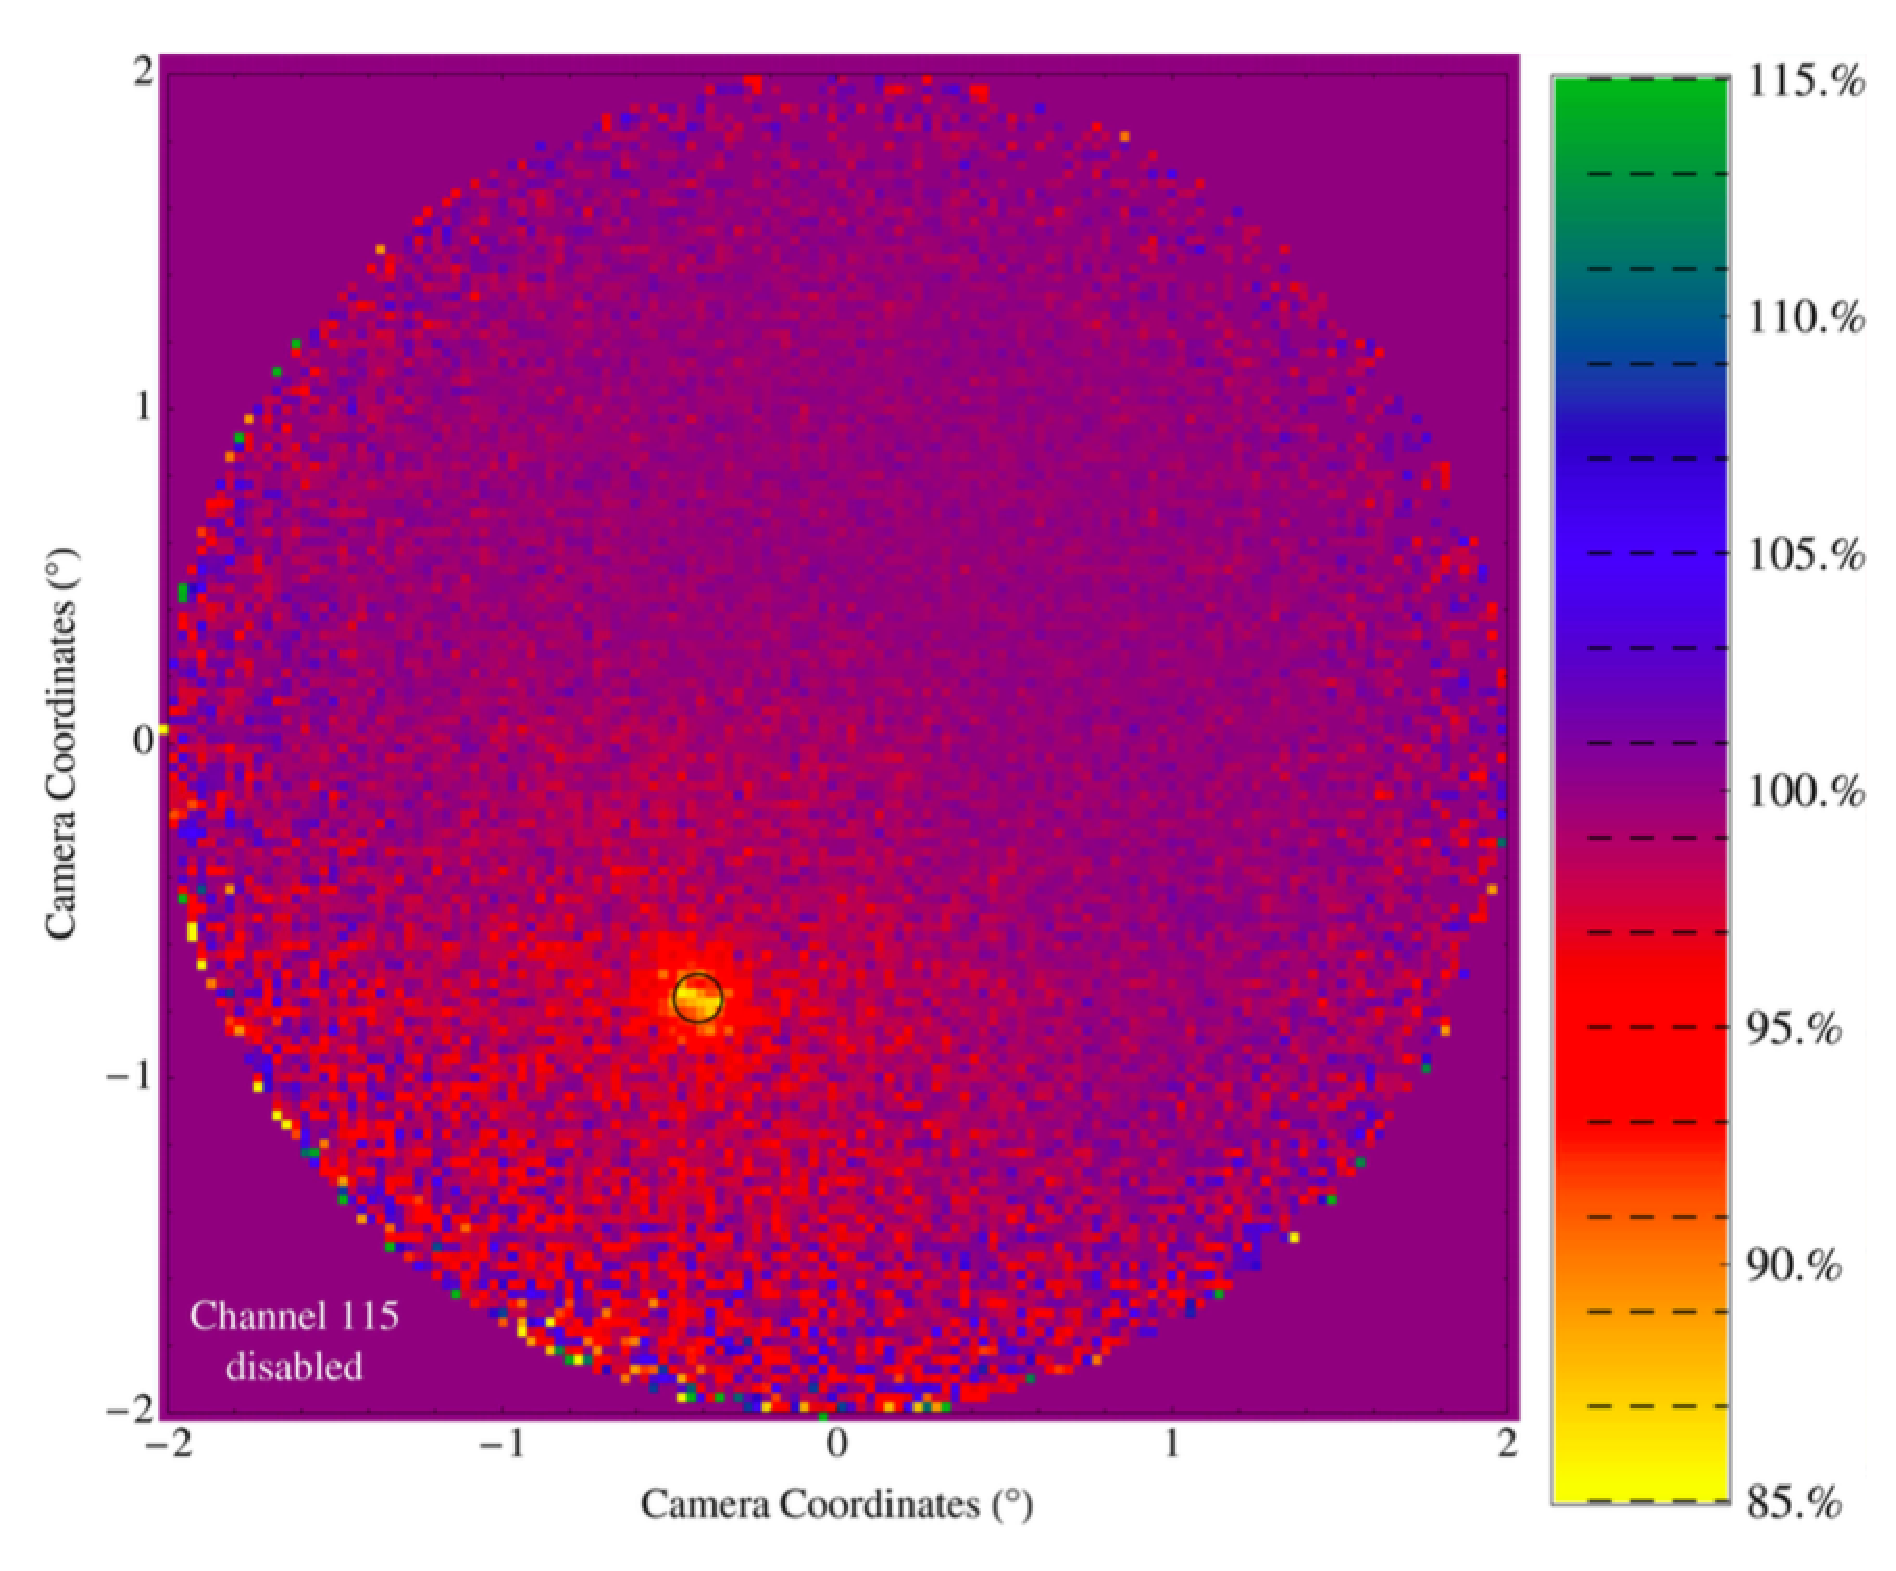
\includegraphics[width=0.8\textwidth]{images/disabled_pixel/relativerate_camera}
      \caption[Relative Event Rate]{
        Event rate in the camera with pixel 115 disabled (denoted by the black circle) in all four telescopes, relative to having all pixels enabled.
        Camera coordinate axes are parallel to azimuth and elevation.
      }
      \label{fig:dpix_rel_camera}
    \end{figure}

    In Figure \ref{fig:dpix_rel_radial}, the bin values from Figure \ref{fig:dpix_rel_camera} are divided into radial bins centered around the disabled pixel.
    The average relative event rate is then calculated for each bin, along with a 1-sigma distribution width for the error bars.
    It can be seen that there are three distinct regions to the plot.
    (How do you actually calculate the uncertainties here? If you take a ratio between numbers of events, you need to calculate the uncertainty explicitly since there are many events which are common to both bins and they shouldn’t be counted twice in the uncertainty.  This is important as it affects the conclusion you reach below. --Orel??)
    In the first region, from radius $\ang{0}$ to $\ang{0.3}$, the relative event rate starts extremely low, and rises rapidly.
    In the second region, from radius $\ang{0.3}$ to $\ang{1.6}$, the relative event rate is still rising, but much more slowly.
    In the third region outside $\ang{1.6}$, there is almost no effect.

    ??This discussion of three regions is not really correct and not entirely relevant.
    It does not give a conclusion on what you do with this information.
    The simplest idea would be to apply a correction to events with disabled pixels based on this plot. Do you that? If not, why not? If yes, it should be mentioned here.
    There are really only two “regions” in this plot, one where you lose events and need to correct for that and one where the ratio is 100% within uncertainties.
    Here is where the correct calculation of uncertainties of the ratio becomes important.
    I think as it is, you might be overestimating the uncertainties, which would result in a larger systematic uncertainties from this correction, if you apply it. --Orel??


    \begin{figure}[ht]
      \centering
      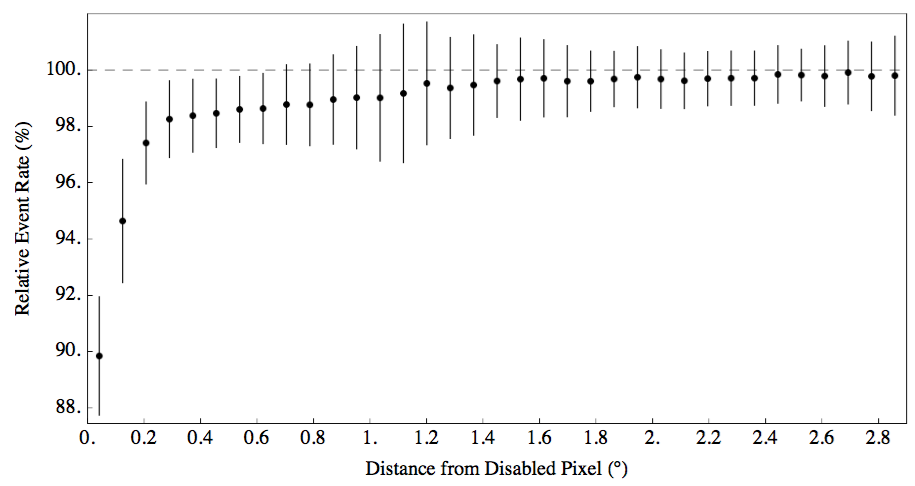
\includegraphics[width=\textwidth]{images/disabled_pixel/relativerate_radial}
      \caption[Radial Relative Event Rate]{
        Same relative event rate as in Figure \ref{fig:dpix_rel_camera}, but averaged into radial bins, centered on the disabled pixel 115.
      }
      \label{fig:dpix_rel_radial}
    \end{figure}

    In Figure \ref{fig:dpix_disappear}, the positions of events that were rejected by cuts are shown.
    The white area indicates many events are lost in the area of the disabled pixel.
    These events would have smaller images, and would be much more susceptable to being cut.

    \begin{figure}[ht]
      \centering
      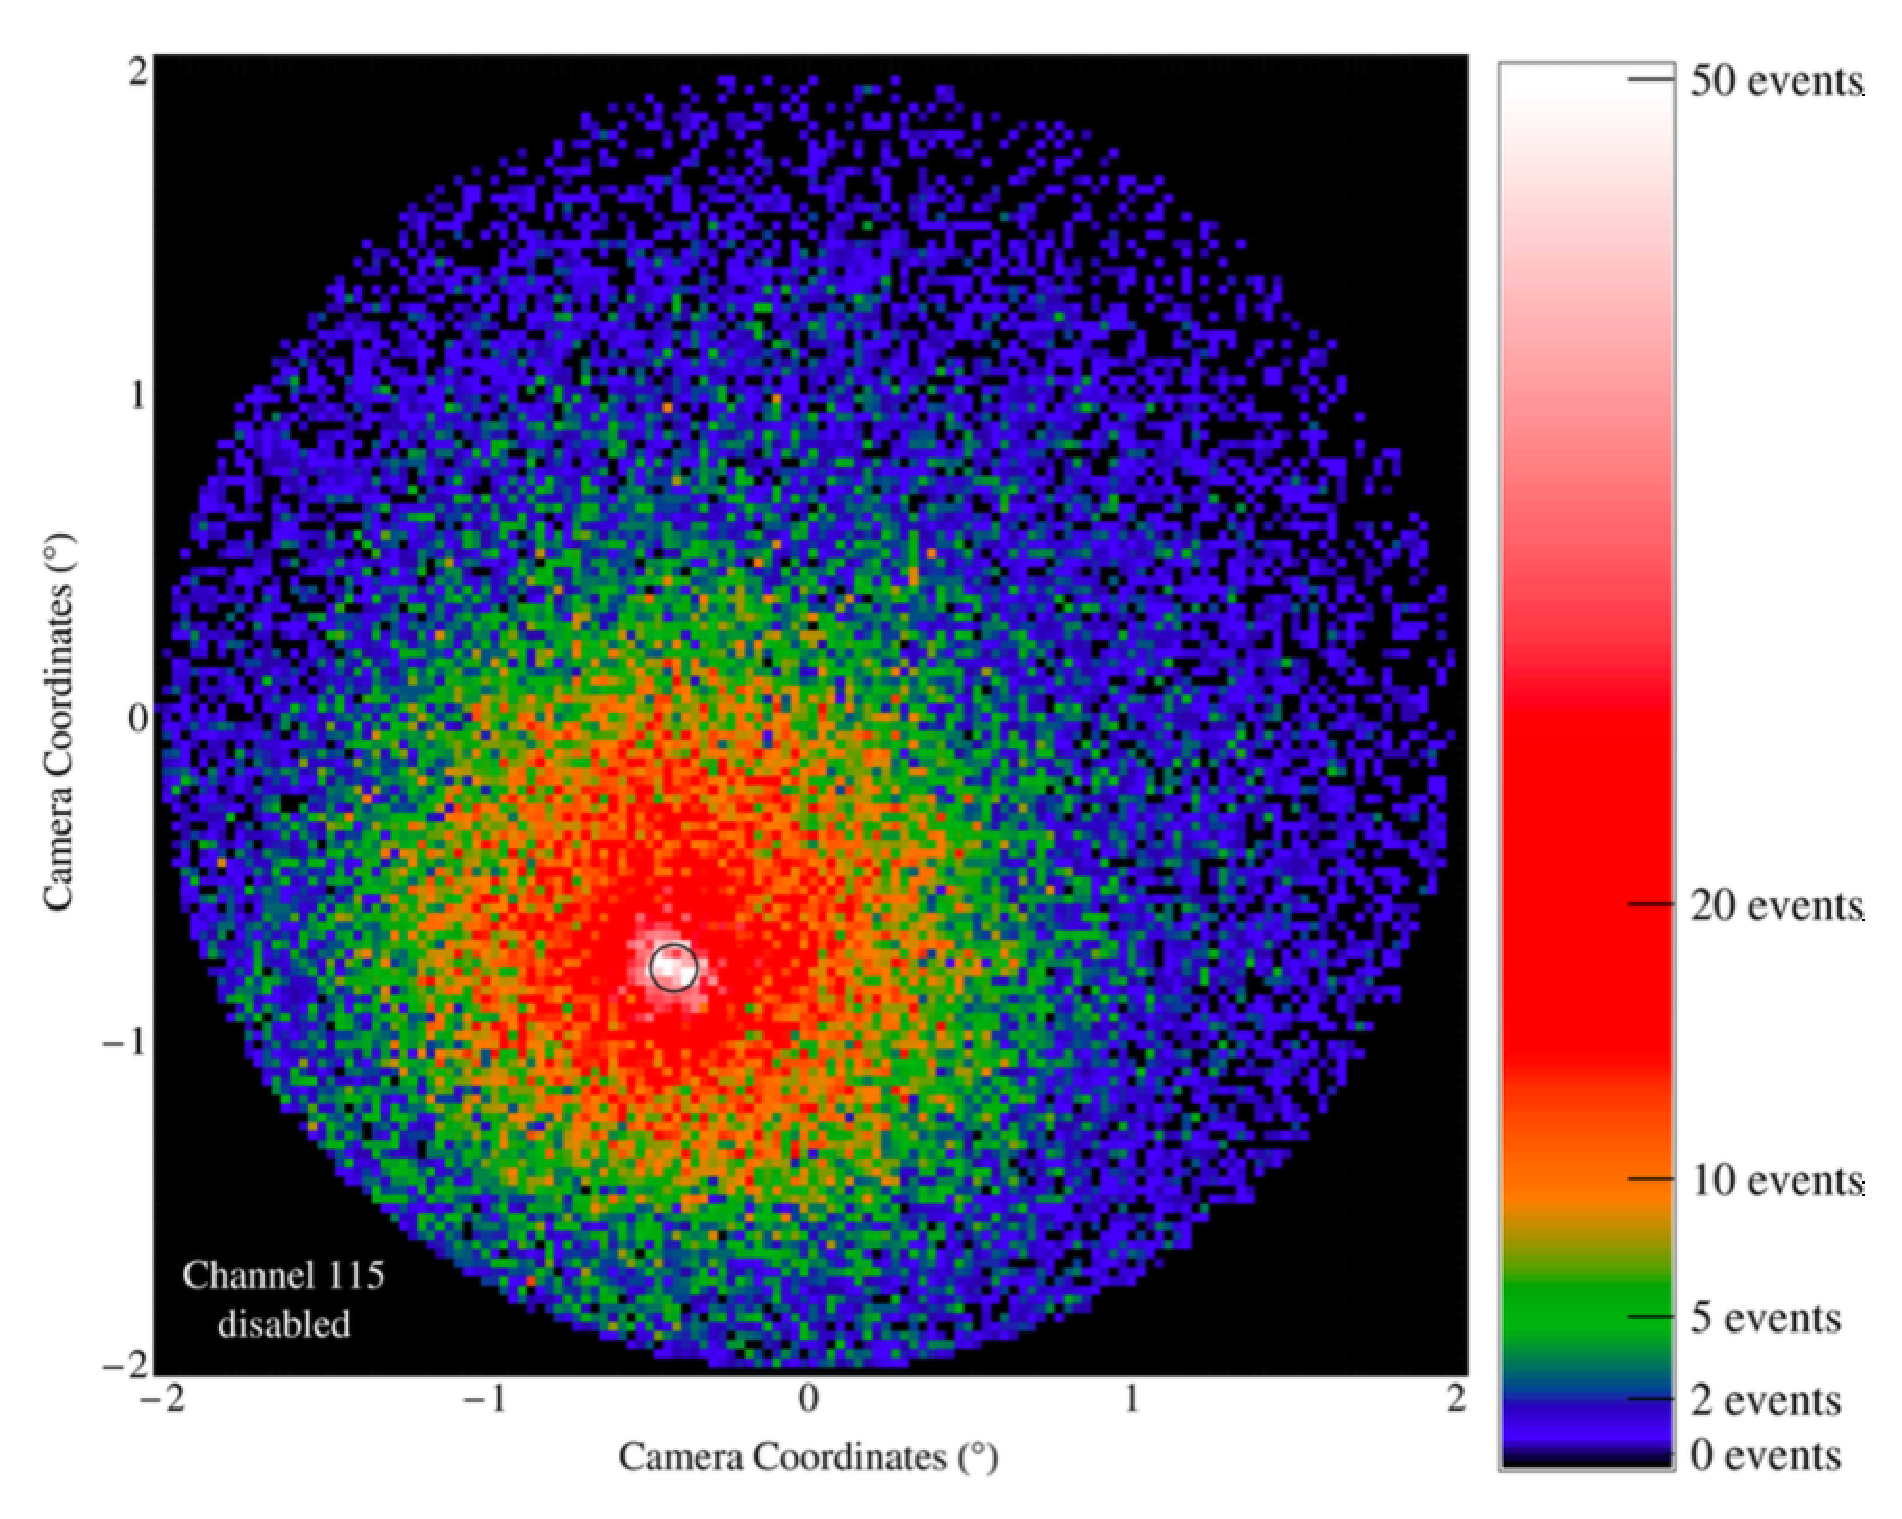
\includegraphics[width=0.8\textwidth]{images/disabled_pixel/disappearing_events}
      \caption[Disappearing Events]{
        Positions of events that disappeared when pixel 115 was disabled in all four telescopes.
        Positions are from their pixel-enabled reconstructed position.
      }
      \label{fig:dpix_disappear}
    \end{figure}

    In Figure \ref{fig:dpix_appear}, the positions of events that are now able to pass cuts are shown.
    It should be noted that these are not events that these are events 'created' by disabling a pixel.
    Rather, they are events that, with the pixel enabled, did not pass cuts.
    Now that the pixel is disabled, they do pass cuts.

    What is also noticeable is that the highest concentration of lost events was in the pixel's area, whereas the highest rate for appearing events is actually in a ring with a radius of \nicetilde1.5 pixels around the disabled pixel.
    This is probably due to the fact that disabling a pixel can make some images look thinner or wider, depending on where the disabled pixel is in the image.
    A thinner image will look more gamma-like, making it more likely to pass cuts, appearing like 'new' events.
    On the other hand, a wider image looks more hadron-like, and is less likely to pass cuts, causing some events to disappear.

    \begin{figure}[ht]
      \centering
      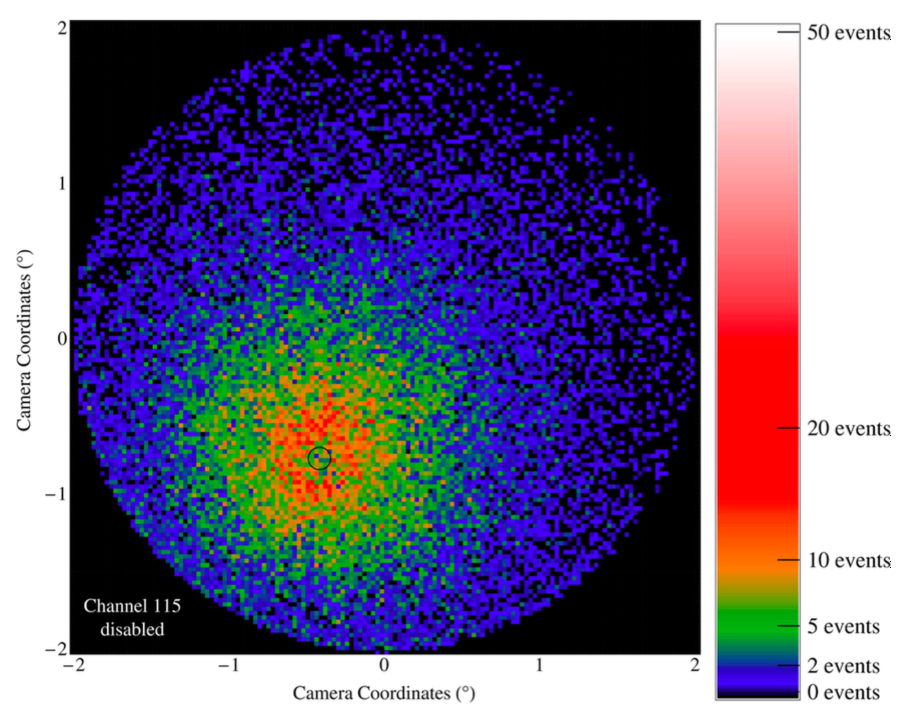
\includegraphics[width=0.8\textwidth]{images/disabled_pixel/appearing_events}
      \caption[Newly Appearing Events]{
        Positions of new events that appeared when pixel 115 was disabled in all four telescopes.
        Positions are from their pixel-disabled reconstructed position.
      }
      \label{fig:dpix_appear}
    \end{figure}

    In Figure \ref{fig:dpix_move}, the movment of gamma-like events is shown, when pixel 115 was disabled in all four telescopes.
    Only events which moved more than $0.1*psf$ are shown.
    It should be noted that relatively few (how few??) events move, and the events that do move are mostly ones with non-compact image shapes that are cut in half when a pixel is disabled.

    What can be learned from this is that while only a small number of events' positions depend on a given pixel, pixels can have an impact on the reconstructed position from halfway across the camera.
    This may imply that the event PSF is, to second order, dependent on the number of disabled pixels, though no studies were done to confirm this.(is it ok to guess this??)


    \begin{figure}[ht]
      \centering
      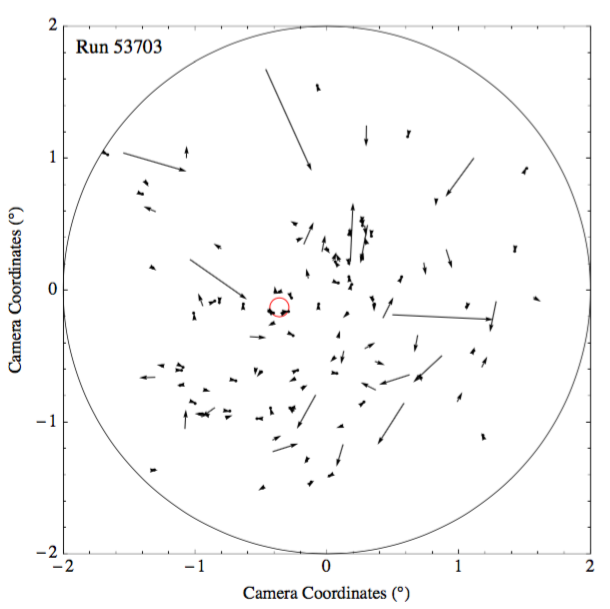
\includegraphics[width=0.8\textwidth]{images/disabled_pixel/moving_events}
      \caption[Event Movement]{
        Positions of events that moved when pixel 115 (denoted by the red circle) was disabled in all four telescopes.  
        Arrows point from the pixel-enabled position to the pixel-disabled position.
      }
      \label{fig:dpix_move}
    \end{figure}

    As the acceptance for a particular event and the event's effective area are strongly related, the loss of acceptance also means a loss of effective area in the area of this pixel.
    This can have effects on the energy reconstruction.

    For CTA, the pixels are ?? set up so that ?? only one pixel will be shut off at a time due to a bright star.
    While this will limit the effect of very bright stars, CTA's planned $\ang{7}$ field of view will mean there are many more stars in view, meaning many more holes to account for.

    Future studies could also compare how events move in energy or time when a pixel is disabled.
    Another study might investigate how the reconstructed shower-telescope distance changes, since a shower with fewer pixels will look further away, and may be reconstructed differently.
    In general, as a pixel is disabled, it is expected that lower energy events and showers further away will be more vulnerable, and will show stronger differences than higher energy events or closer showers.


